%Preamble
\documentclass[11pt,oneside,letterpaper]{article}

% text layout
\usepackage{geometry}
\geometry{textwidth=15cm} % 15.25cm for single-space, 16.25cm for double-space
\geometry{textheight=22cm} % 22cm for single-space, 22.5cm for double-space

% make links a more pleasing color and don't box them
\usepackage{color}
\definecolor{green}{rgb}{0.20,0.50,0.48}
\usepackage[hidelinks]{hyperref}
\hypersetup{colorlinks=true,linkcolor=black,citecolor=black,urlcolor=green}

\usepackage{parskip}

\usepackage{authblk}
\usepackage[utf8]{inputenc}
\usepackage[T1]{fontenc}
\usepackage{amsmath}
\usepackage{amssymb}
\usepackage{amsthm}
\usepackage{amsfonts}
\usepackage{mathrsfs}
\usepackage{mathtools}
\usepackage{enumerate}
\usepackage[shortlabels]{enumitem}
\usepackage{verbatim} %% includes comment environment
\usepackage[capitalize]{cleveref}
\crefformat{equation}{~(#2#1#3)}
\usepackage{graphicx}
\usepackage{mathrsfs}

% cite package, to clean up citations in the main text
\usepackage{cite}

% bold the 'Figure #' in the caption and separate it with a period
% Captions will be left justified
\usepackage[labelfont=bf,labelsep=period,font=small]{caption}

% can include this for journal submission to help with reviewer feedback, but don't include for preprint
% \usepackage{lineno}
% \linenumbers
% \linespread{1.5} % Increase Line spread

\renewcommand{\vec}[1]{\boldsymbol{#1}}

\title{SARS-CoV-2 variant dynamics across US states show consistent differences in effective reproduction numbers}

\author[1,2,*]{Marlin D.\ Figgins}
\author[1,3]{Trevor Bedford}
\affil[1]{Vaccine and Infectious Disease Division, Fred Hutchinson Cancer Research Center, Seattle, WA, USA}
\affil[2]{Department of Applied Mathematics, University of Washington, Seattle, WA, USA}
\affil[3]{Howard Hughes Medical Institute, Seattle, WA, USA}
\affil[*]{Corresponding author: mfiggins@uw.edu}
\date{\today}
%Figure out author affilations...
% https://maehler.se/blog/2013/11/01/authors-and-affiliations-in-latex

\begin{document}

%TODO: Focus on synthesizing literature in the discussion to discuss limitations and future directions
%TODO: What should two sentence takeaway be if I had to explain this to someone who was familiar with this line of work?

\maketitle

\begin{abstract}
Accurately estimating relative transmission rates of SARS-CoV-2 Variant of Concern and Variant of Interest viruses remains a scientific and public health priority.
Recent studies have used the sample proportions of different variants from sequence data to describe variant frequency dynamics and relative transmission rates, but frequencies alone cannot capture the rich epidemiological behavior of SARS-CoV-2.
Here, we extend methods for inferring the effective reproduction number of an epidemic using confirmed case data to jointly estimate variant-specific effective reproduction numbers and frequencies of co-circulating variants using case data and genetic sequences across states in the US from January to October 2021.
Our method can be used to infer structured relationships between effective reproduction numbers across time series which may be amendable to various analyses including other features related to the effective reproductive number such as non-pharmaceutical interventions or build up of population immunity.
We use this model to estimate the effective reproduction number of SARS-CoV-2 Variants of Concern and Variants of Interest in the United States and estimate consistent growth advantages of particular variants across different locations.

%TODO: Sentence about growth advantages
%TODO: Sentence about the applicability of this method generally
\end{abstract}

\section*{Introduction}


%TODO: Lead into the pandemic, thorough descriptions on how genetic differences in variants may lead to different outcomes at the level of transmission and clinical presentation.
%TODO: Move into the specifics of SARS-CoV-2. What info does a reader 2 years from now need to know to be able to make sense of this work?
%TODO: Mention that modeling efforts are useful for understanding what has happened over the course of the pandemic.
%TODO: And will be useful for tackling the continued spread of SARS-CoV-2

As SARS-CoV-2 evolves, variants may emerge that increase in their ability to transmit and escape acquired immunity \cite{tao2021biological}.
Quantifying the observed growth advantages of SARS-CoV-2 variants allows us to understand which variants are able to thrive in different locations \cite{tegally2021detection, davies2021estimated}.
Relating genomic data of SARS-CoV-2 lineages to epidemic surveillance data is difficult.
Although it is typical to use phylodynamic methods to analyze genetic sequence data from epidemics, the sheer amount of data as well as challenges to describing fitness effects in phylodynamic models make these methods hard to apply to potential differences in transmission rate among circulating variants.
In order to deal with the limitations of phylodynamic inference, previous studies have estimated the growth of lineages using observed frequencies in sequenced SARS-CoV-2 samples \cite{Annavajhala2021, Faria2021, Obermeyer2021, Ito2021}.
Such methods often model the frequency of lineages using multinomial logistic regression \cite{Ito2021, Obermeyer2021}, which generally assumes that genetic variants have a fitness advantage over one another which is fixed in time and acts as a estimate for the selective advantage of different variants at the level of frequencies.
Although a consistent increase in frequency of one variant over another is expected to reflect differences in transmission rate, these models do not directly account for the complicated infection and transmission dynamics which influence which variants lead to local and regional epidemics.
When dealing with competition between variants, variants which are declining in frequency can still lead to an increasing number of infections.
Similarly, growth in frequency does not necessarily entail an increase in absolute infections.

To better capture epidemiological dynamics, there are methods which describe the growth in number of infections using confirmed case, hospitalization, or death data to estimate changes in the effective reproduction number $R_{t}$, the average number of infections a single infectious individual generates, during a given outbreak.
Although these methods are excellent for describing overall epidemic growth rates, they cannot capture the evolutionary dynamics and fitness changes between different variants since they often assume the population dynamics are described by a singular $R_{t}$ trajectory \cite{Cori2013, Abbott2020}, which internally is unrelated to the genetic and phenotypic composition of the population.
This is of particular importance in the analysis of an epidemic in which a dominant lineage may be declining overall, but some sublineage is rapidly increasing in frequency and absolute prevalence, creating the potential for a secondary wave of infections that may go unnoticed at first glance.
To overcome this we require models that partition case counts into contributions from different variants to estimate variant-specific effective reproduction numbers.

The current COVID-19 pandemic serves as an important example of this phenomenon.
After initial emergence in late 2020, over the course of 2021, Variant of Concern (VOC) and Variant of Interest (VOI) viruses spread throughout the world and replaced existing viral diversity.
Multiple WHO designated \cite{Konings2021} VOC and VOI viruses circulated in spring and early summer 2021, but this diversity was largely replaced by Delta variant viruses which became globally dominant in late summer 2021.
Although it's now clear that Delta had greater transmissibility than other variants, rigorous estimates of the relative fitness of circulating VOC and VOI viruses are of interest.
Here, we develop a joint epidemiological and population genetic model of SARS-CoV-2 to assess the growth of different variants over time and infer differences in the effective reproduction numbers of SARS-CoV-2 variants as well as underlying frequency of variants under noisy sampling.
We apply this model to sequence data and case count data from United States between January and October 2021 to estimate differences in transmissibility between circulating VOC and VOI viruses.

\section*{Results}

\paragraph{Model Overview}%

\begin{figure}[h!]
  \centering
  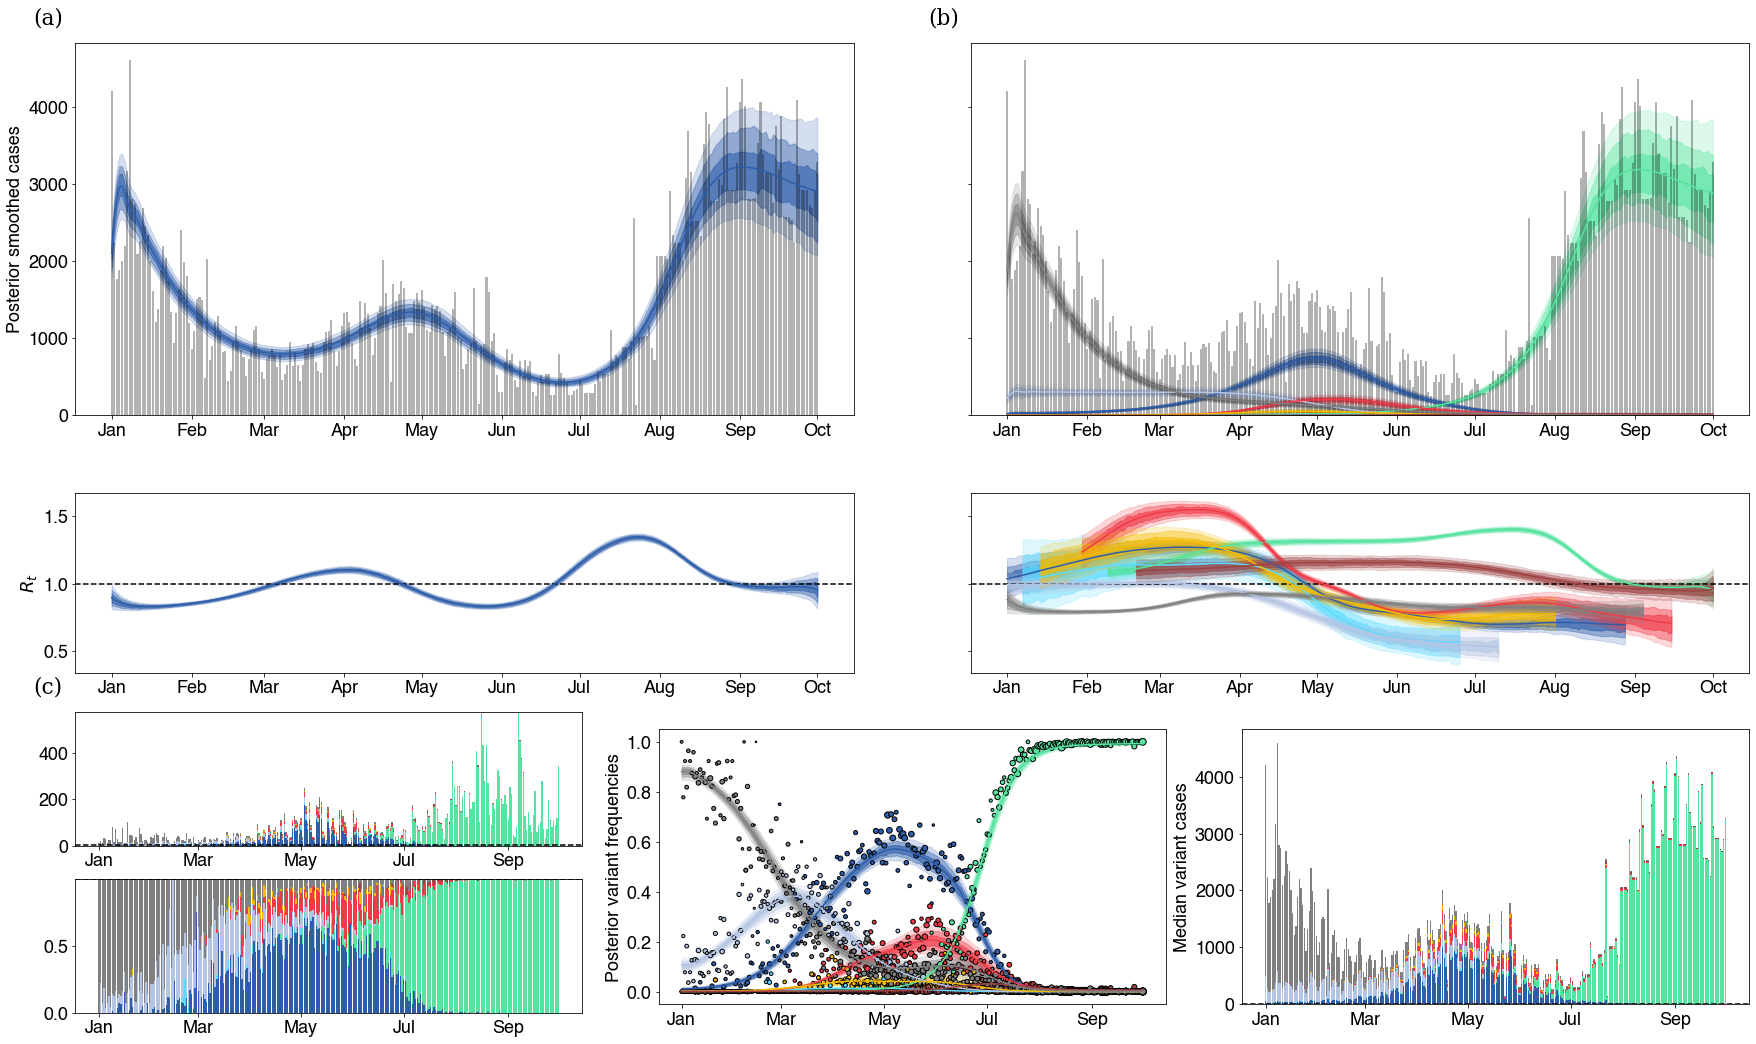
\includegraphics[width=\linewidth]{figs/free_rt_Washington.png}
  \caption{\textbf{Fitting the free $R_{t}$ model to Washington state data.}
    (a) When assessing epidemic growth rates, we often compute a single effective reproduction number trajectory which is effectively an average over the all viruses in population.
    Gray bars are observed daily case counts, while blue lines are model inferences with 50\%, 80\% and 95\% credible intervals.
    (b) Epidemics are made of different variants which may differ in fitness. Using case counts alongside sequences of different lineages allows us to understand the proportion of different variants in the population.
(c) Using both case count and frequency data, we can estimate the effective reproduction numbers of different lineages.}%
  \label{fig:free_rt_Washington}
\end{figure}

\begin{figure}[h!]
  \centering
  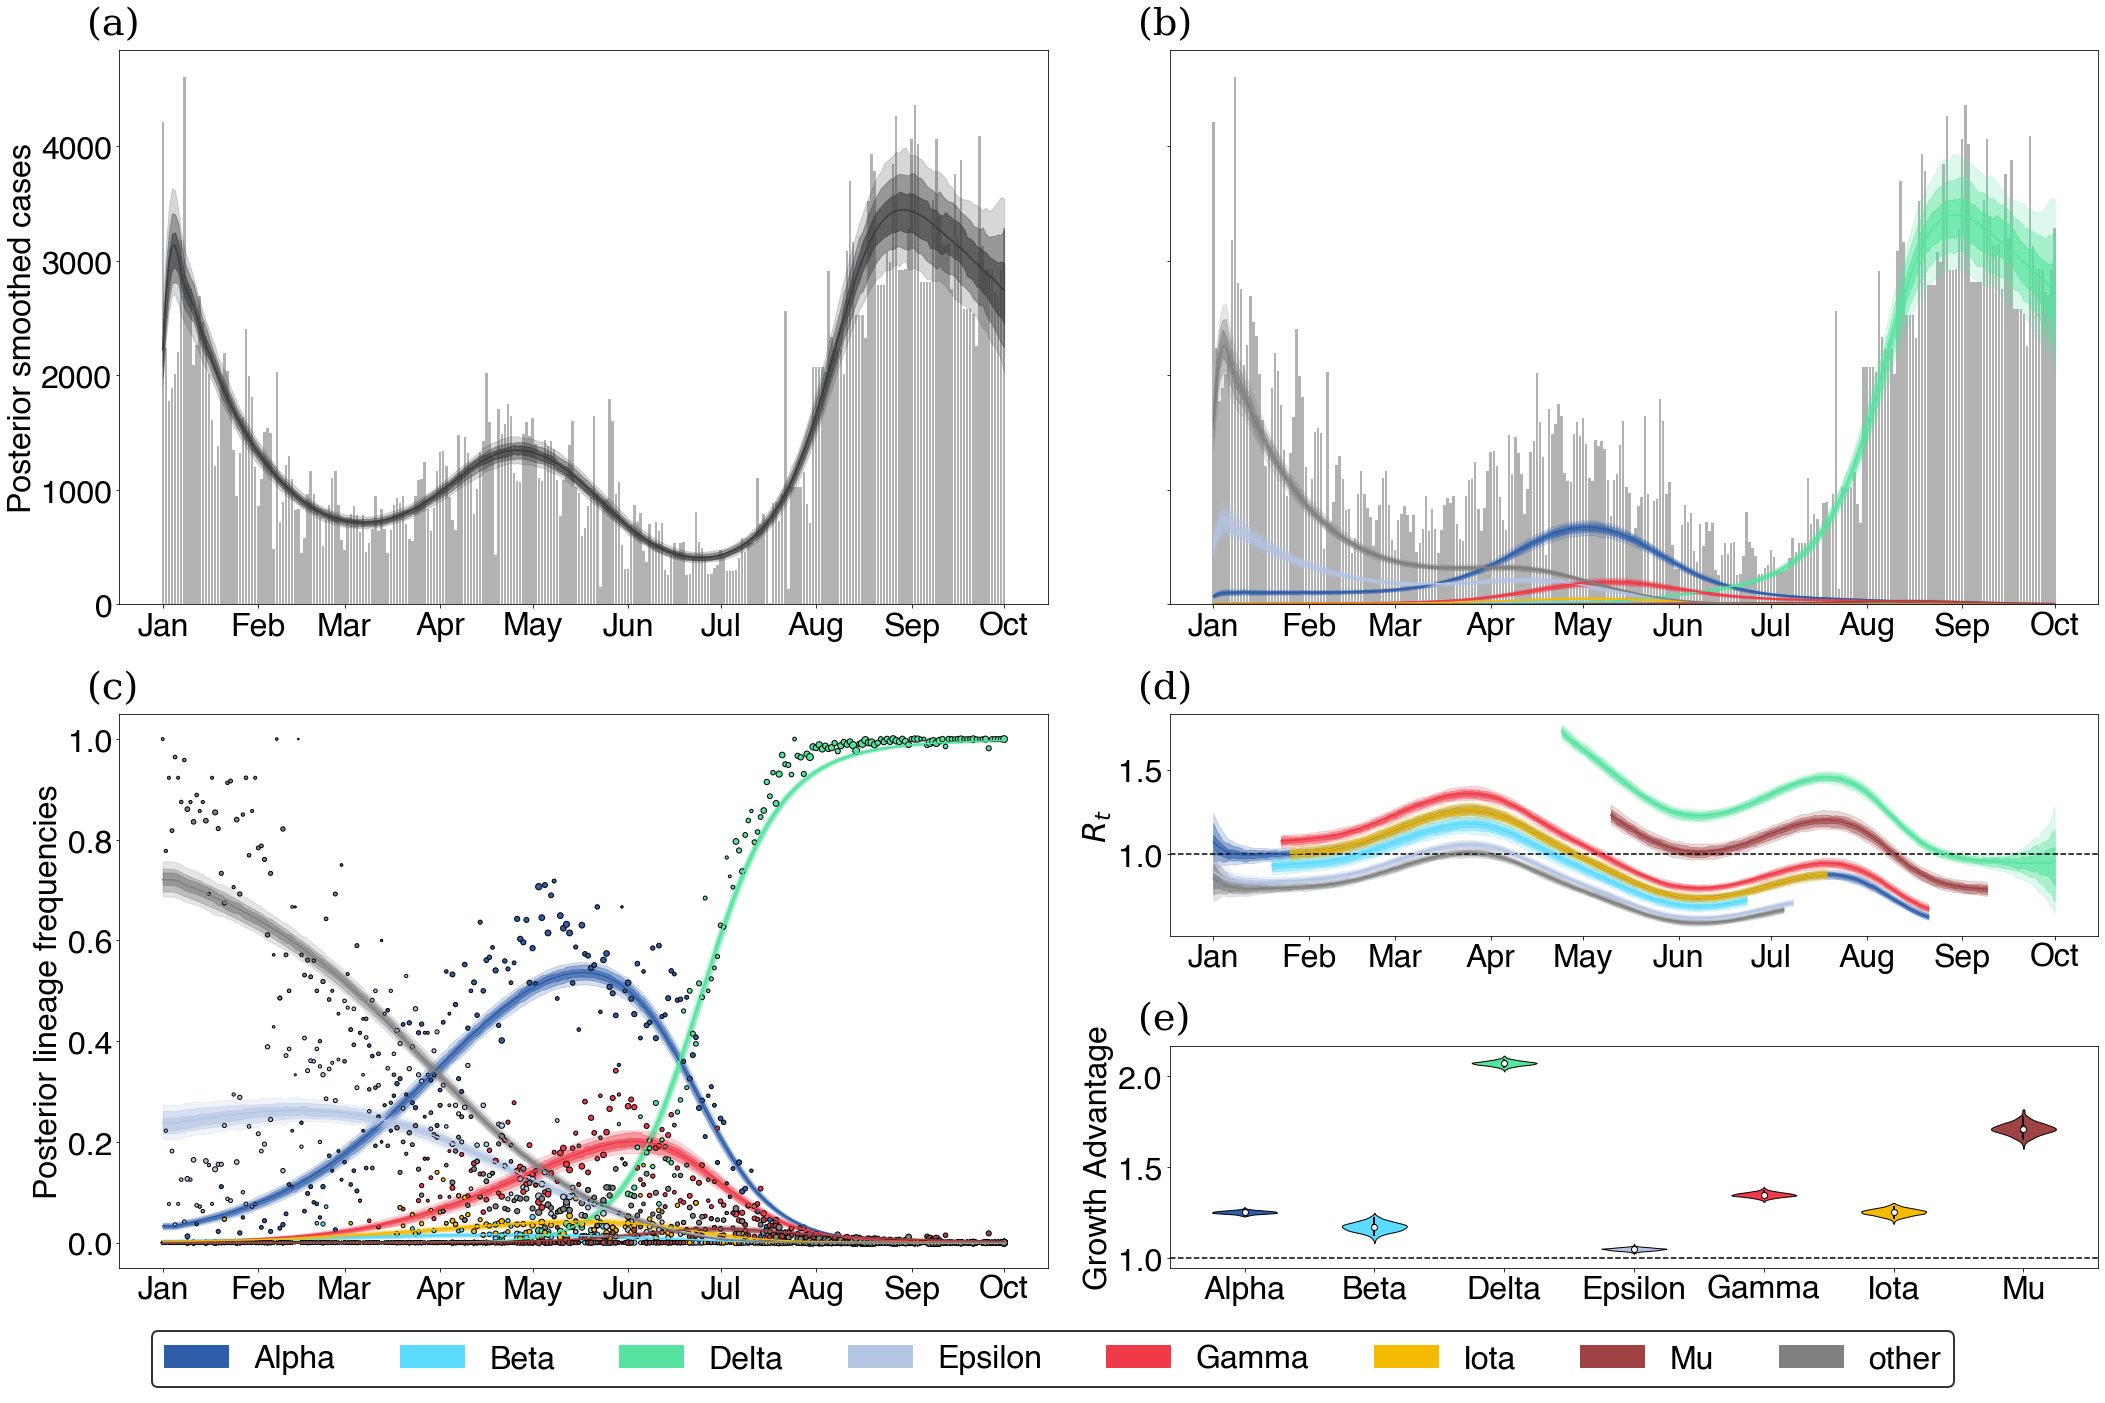
\includegraphics[width=\linewidth]{figs/fixed_growth_Washington.png}
  \caption{\textbf{Fitting the fixed growth advantage model to Washington state data.}
  (a) Posterior expected cases without weekly seasonality in reporting rate.
  Gray bars are observed daily case counts, while blue lines are model inferences with 50\%, 80\% and 95\% credible intervals.
  (b) Posterior expected cases by lineage.
  Each colored lines is a different variant with intervals of varying opacity showing 50\%, 80\% and 95\% credible intervals.
  (c) Posterior lineage frequency against observed sample frequency.
  Dots represent observed weekly frequencies in sequence data and each colored line is a different variant with shaded CIs.
  (d) Variant-specific effective reproduction numbers.
  (e) Posterior growth advantage by variant.}
  \label{fig:fixed_growth_Washington}
\end{figure}

We implement two models of variant-specific effective reproduction number based on a renewal equation framework of epidemic spread (see Methods), a free $R_{t}$ model and a fixed growth advantage model.
These models assume that new infections are determined by two essential parameters: the effective reproduction number which determines the average number of secondary infections generated over the course of a primary infection and the generation time which determines length of infection as well as their relative transmissibility over the course of their infection.
In both models, variants generate infections independently of one another, but the sum of infections across variants is observed through surveillance data like case counts or hospitalizations.
In order to disaggregate infections by variant we rely on frequency estimates which are informed by counts of sequenced samples using a Dirichlet-multinomial likelihood.

The transmission of each variant is modeled using a deterministic renewal equation which allows for realistic delay distributions between infection, transmission, and detection as a case.
With this approach, we need only to determine the initial number of infections and the variant-specific effective reproduction numbers to estimate the frequency of each variant in the population over time.
Due to this, the differences between the two models is determined in how each parameterizes variant-specific effective reproduction numbers.

In the first model, we introduce a free variant $R_{t}$ which infers the effective reproduction number of each variant independently from one another to allow for non-linear relationships between the growth rates of different variants over time.
Each variant effective reproduction number is parameterized using an exponentiated spline basis, so that the log effective reproduction numbers are described by a linear basis expansion.

The second model is a fixed growth advantage model of variant $R_{t}$ in which each variants has its own multiplicative growth advantage which acts as a scaling to a single non-variant $R_{t}$ trajectory.
With this fixed growth advantage model, we parameterize fitness of variants at the level of transmission by inferring variant-specific effective reproduction numbers.
This differs from previous work on variant effective reproduction numbers which often parameterize these differences by assuming logistic growth of frequencies \cite{Earnest2021, Vhringer2021}.
Though, in general, our method allows one to estimate variant growth in the frequency domain in terms of effective reproduction number differences, we find that assuming a fixed advantage for variants results in estimates which are qualitatively similar to the aforementioned models which assume fixed growth advantages in frequency growth.
This provides the additional benefit of the inferred parameters being interpretable as scaling the effective reproduction number.

In cases where a singular fixed growth advantage is insufficient to describe the data, we return to our first model in which the effective reproduction numbers of variants are modeled without assuming a fixed advantage, accounting for possible variation in variants' advantages over one another over time.

We demonstrate these models on data from Washington State.
The free $R_{t}$ model is shown in Figure \ref{fig:free_rt_Washington} and the fixed growth advantage model is shown in Figure \ref{fig:fixed_growth_Washington}.
% Example model output from several other states is provided in the supplemental materials. TB: Will add this back once there are references to supp figures in Supp Materials.

\begin{figure}[t]
  \centering
  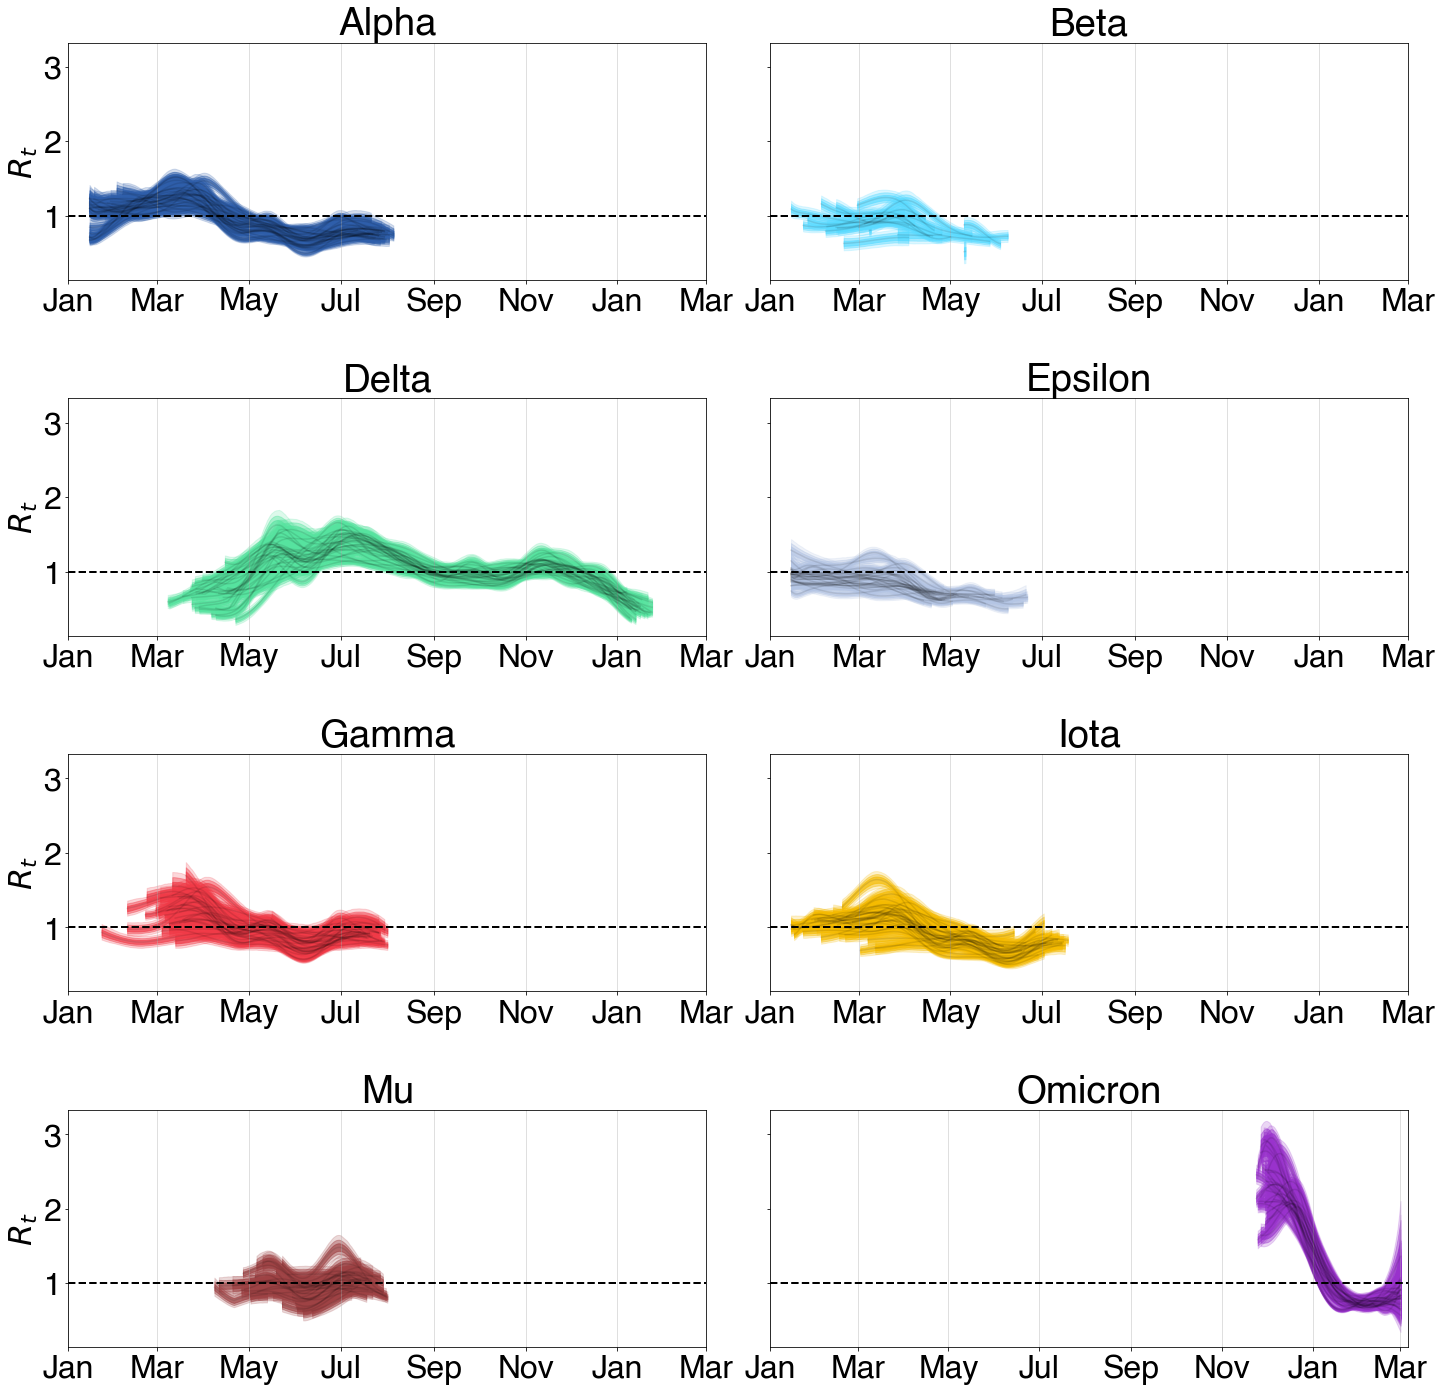
\includegraphics[width=\linewidth]{figs/rt_consensus.png}
  \caption{\textbf{Inferred effective reproduction numbers from free $R_t$ model in 39 states show consistent trends of variants across states.}
  Each panel shows a series of 39 trajectories, representing $R_t$ through time for this variant across states.
  Shaded intervals show 50\%, 80\% and 95\% credible intervals.
  }
  \label{fig:rt_consensus}
\end{figure}

\paragraph{Estimating growth advantages in the United States}

We estimate the effective reproduction numbers of SARS-CoV-2 Variant of Concern and Variant of Interest viruses in the United States using daily confirmed case counts obtained from the US CDC and sequence counts annotated by variant obtained from the Nextstrain-curated `open' dataset \cite{Hadfield2018} (see Data and code accessibility).
Each sequence is labeled with a Nextstrain clade \cite{Hadfield2018} and we partition clades into variants based on designated WHO VOC/VOI status \cite{Konings2021}.
Nextstrain clades annotated in the fashion correspond to a subset of major lineages designated by PANGO \cite{Rambaut2020}.
We consider the following 7 variants which have been flagged as variants of interest or concern and which circulated in the US during 2021: Alpha (PANGO lineage B.1.1.7, Nextstrain clade 20I), Beta (lineage B.1.351, clade 20H), Gamma (lineage P.1, clade 20J), Delta (lineage B.1.617.2, clade 21A), Epsilon (lineage B.1.427/429, clade 21C), Iota (lineage B.1.526, clade 21F), and Mu (lineage B.1.621, clade 21H).
We use a cutoff of 2000 sequences from a particular variant across states to determine threshold of circulation.
This eliminates Eta, Lambda, Kappa and Theta from consideration and groups these variants along with ancestral `non-variant' viruses into a single `other' category.
We use a cutoff of 5000 sequences from a particular state as basis for including the state in the dataset.
This cutoff left 39 states available for inference.

\begin{figure}[t]
  \centering
  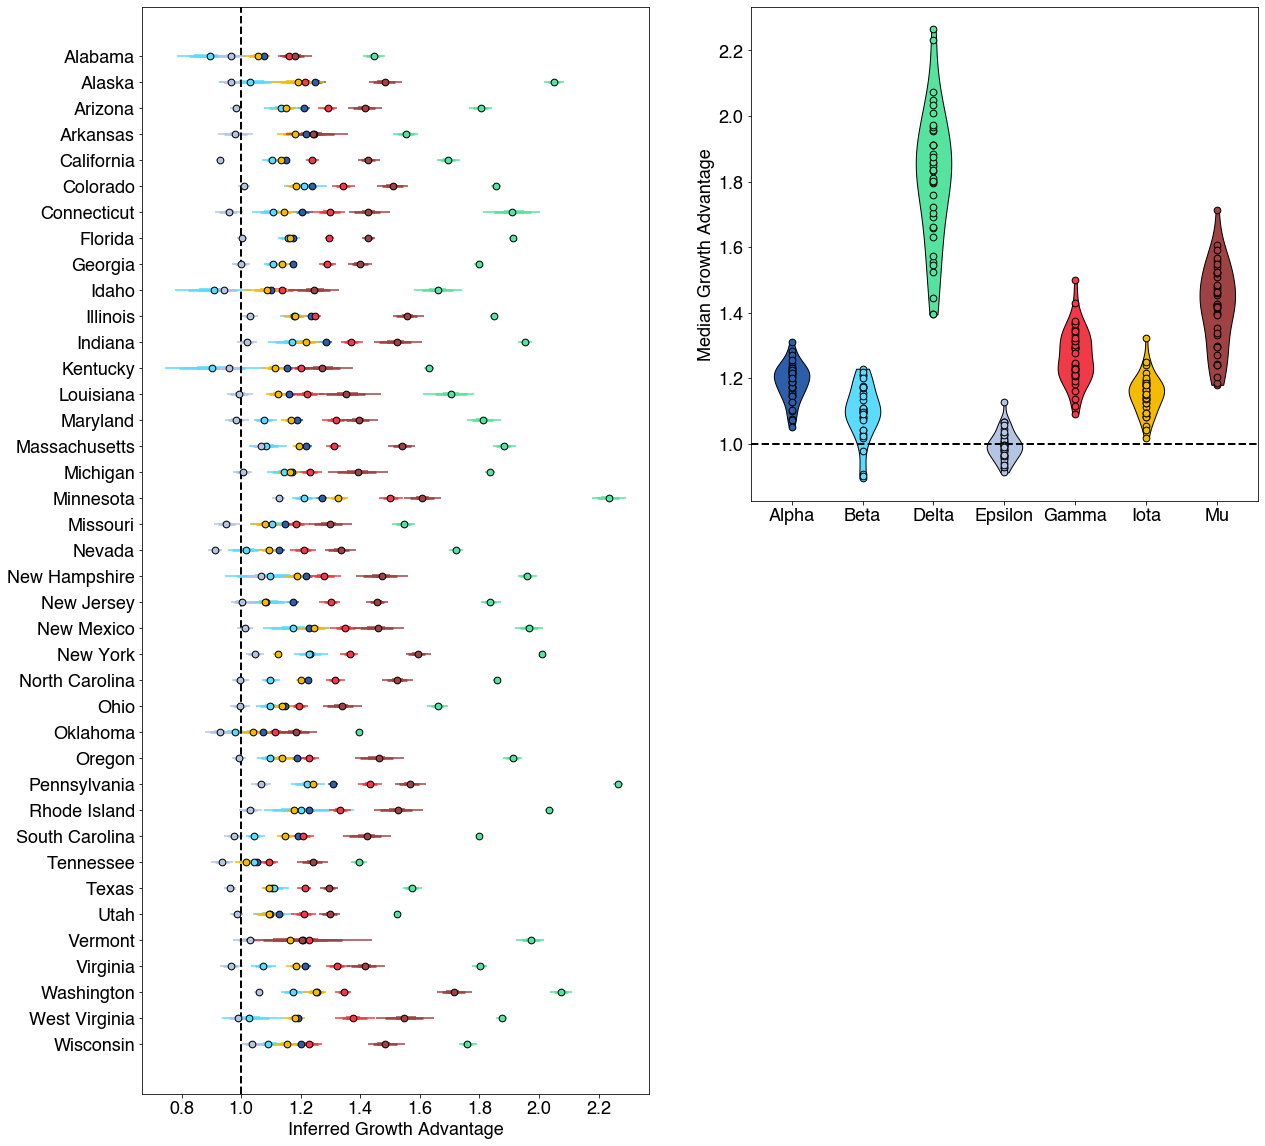
\includegraphics[width=\linewidth]{figs/growth_advantages.png}
  \caption{\textbf{Using fixed growth advantage model, we infer growth advantages for 7 variants in 39 US states.}
  (a) Growth advantages for variants of concern. Each point is the median growth advantage inferred from a single state.
  (b) Same as (a) but visualized by variant.}
  \label{fig:growth_advantages}
\end{figure}

In order to inform our estimates of the frequency of genetic variants, we divide sequences from each state into daily sample counts for each of the 7 variants above and a single `other' category.
We then use these counts alongside the daily case counts in each state to estimate the effective reproduction number for individual variants using our free $R_{t}$ model.
We find that overall there appears to be consistent trends in the effective reproduction numbers of variants across the United States (Fig.\ \ref{fig:rt_consensus}).
We see that non-variant viruses were declining from January onwards, while initial VOCs Alpha and Gamma initially had $R_t>1$, but saw $R_t$ decline below one across most states in April and May respectively.
Upon arrival in May, Delta shows significantly higher values of $R_t$ that don't decline below 1 until September.

In order to transform these observed trends to a variant-specific growth advantage, we rely on our fixed growth advantage model which infers a fixed variant-specific growth advantage as a multiplicative scaling of the effective reproduction number.
Using the fixed growth advantage model, we find that most variants identified share some positive growth advantage with the exception of Epsilon.
Further, these growth advantages appear to be consistent between the states analyzed (Fig.\ \ref{fig:growth_advantages}).
Alpha, Beta, Gamma and Iota show modest growth advantage over largely ancestral `other' viruses, while Mu and Delta show larger growth advantages.
Mu has previously been associated with increased neutralization resistance to convalescent serum \cite{Uriu2021}, and its advantage of 1.2--1.8 across states is perhaps partially driven by immune escape.
Despite this, Mu's growth advantage whether from immune escape or otherwise was insufficient to outcompete Delta in any of the states analyzed.
Delta's advantage of 1.6--2.0 across states is particularly significant.
Given this large growth advantage was evident in May (Fig.\ \ref{fig:rt_consensus}), Delta's rapid rise in frequency and sizable epidemic should have been clear at the time.
The significant growth advantage observed in Delta is recapitulated in other studies including Obermeyer et al.\ \cite{Obermeyer2021} and V\"ohringer et al.\ \cite{vohringer2021genomic}.

%TODO: Include particulars about what we learned about individual variants above
%TODO: What are the actual numbers?

\section*{Discussion}

%TODO: Perhaps, main technical takeaway is that you can augment models of frequency dynamics with an epidemiological model of your choosing to relate frequency dynamics to transmission dynamics.
%TODO: Towards composable modeling of genetic variants

We find that a model that partitions case count data based on variant frequency in sequence data works well to describe SARS-CoV-2 variant dynamics in the United States from January to October 2021.
In each state, spring waves are primarily driven by the arrival of Alpha, Beta, Gamma, and Iota variants.
However, as these waves are subsiding, the arrival of Delta with a significantly greater growth advantage, drives a large summer wave.
Importantly, we can directly estimate a variant-specific $R_{t}$, which for example, shows that Delta was a growing rapidly sub-epidemic across states in May, before its impact was noticeable in overall case counts.
We imagine that this general approach could provide early warning of imminent epidemics driven by low-frequency but highly transmissible variants.

With this mind, this work is not without limitations.
The underlying transmission model is deterministic and does not account for demographic stochasticity and over-dispersion in transmission which has been documented in SARS-CoV-2 transmission \cite{Wong29416}.
As with all methods which depend on parameterizations of the generation time, misspecification of the generation time can be lead to biased estimates of the effective reproduction number or growth advantages \cite{Gostic2020}.
In order to quantify this source of error, we derive an equation relating our inferred growth advantages, the epidemic growth rates, and the mean and standard deviation of the generation time distribution (see Supplemental Appendix).
There is also a general need to account for biases in the case data which may not faithfully describe the infection dynamics of SARS-CoV-2 due to changes in case ascertainment rate, as possibly caused by differences in testing intensity, infection severity among other reasons.
However, we suspect that case ascertainment remained largely consistent from January to October 2021.

We do not explicitly model multiple introductions of variants which can play an important role in variants establishing themselves in different geographies at low infection counts and could bias our estimates of the effective reproduction number if not properly accounted for \cite{Cori2013, MullerWagner2021}.
This could be especially impactful early on when variant cases are driven by multiple importations from a large epidemic elsewhere in the world.
However, we expect once local transmission is predominant that estimated $R_{t}$ will reflect characteristics intrinsic to the variant in the local geography.
Using hierarchical models of variants to jointly estimate growth advantages and pool estimates across locations could be a useful approach for analyzing consistency between growth advantages of variants geographically and beginning to combat the issue of multiple introduction events.
That said, fully combating this issue would likely involve incorporating demographic stochastic into the model at the level of transmission and reduce its speed of inference, scalability, and limit available inference options.

Although there are several ways to improve these methods and expand their applicability, our current model does have utility as a way of assessing early claims of variant advantages and is able to show there is evidence of consistent variant advantages shared between different geographies.
Additional work is needed to attribute these inferred advantages to biological mechanisms like immune escape and transmissibility \cite{tao2021biological}.
Modeling the effect of changes in other factors such as contact patterns or non-pharmaceutical interventions can be done with the current formulation of the model by including quantities of interest as features in the $R_{t}$ model as in Sharma et al.\ \cite{Sharma2021}.

In general, the development of methods which can account for fitness differences between genetic variants is much needed in order for proper epidemic preparedness.
Our method provides one way of analyzing the growth rates of SARS-CoV-2 variants without directly parameterizing how variants grow in terms of frequency by instead focusing on differences in the effective reproduction number.
In cases where the assumption of a fixed growth advantage is warranted and justified, our fixed growth advantage model provides a way of quantifying variant growth advantages at the level of transmission which allow for various delays between infection, transmission, and sampling.

Our method can be extended to analyze the role of specific constituent mutations defining a variant or lineage in changing the effective reproduction number of specific variants directly, similar to the model formulation of Obermeyer et al.\ \cite{Obermeyer2021}.
With this in mind, our method potentially has use for evolutionary forecasting of variants for SARS-CoV-2 as we inform the frequency dynamics of co-circulating variants by describing their population-level transmission dynamics.
Extending the model further towards this aim will require methods for quantifying population immunity as well as escape potential for circulating and emerging SARS-CoV-2 variants.

With these issues in mind, surveillance of variants should be folded into standard epidemiological surveillance as knowledge of variant-specific growth advantages will be useful for forecasting growth of cases, hospitalization, deaths, vaccine effectiveness among other key metrics related to epidemic response.

\section*{Methods}

Using sampled counts of sequences from different lineages as well as case data, we can infer jointly infer the proportion of variants in the larger population and the effective reproduction number of these variants.

\paragraph{Modeling the infection process}%

We estimate the effective reproduction number of competing lineages using a deterministic renewal equation based framework. These equations arise as the expectation of a Bellman-Harris branching process \cite{Bellman1948} which is a type of Branching process in which offspring generation depends on the age of infection.

The renewal equation framework allows one to model infection processes in a way that is mathematically equivalent to standard epidemic models like the SEIR compartment model \cite{Champredon2018}, but in a way that can be more suitable for estimating the effective reproduction number and forecasting using arbitrary generation times. This renewal equation can be written as
\begin{equation}
  I(t) = R_{t} \int_{0}^{t} I(\tau)g_{t-\tau} d\tau,
\end{equation}
where $g$ is the generation time.
In addition, we also include onset distribution $o$ for symptoms which allows us to compute the prevalence, or the number of active infections, as
\begin{equation}
  P(t) = \int_{0}^{t} I(\tau) o_{t-\tau} d \tau.
\end{equation}
We bin the generation time $g$ and the onset distribution $o$ to nearest day, so that we estimate the daily incidence $I(t)$ and prevalence $P(t)$ as

\begin{align}
  I(t) &= R_{t} \sum_{\tau < t} I(\tau) g_{t-\tau}\\
  P(t) &= \sum_{\tau < t} I(\tau) o_{t-\tau}
\end{align}

We parameterize the generation time $g$ as having Gamma distribution with mean 5.2 and standard deviation 1.72 in line with the estimates of \cite{Ganyani2020} and onset time $o$ as having LogNormal with mean 6.8 and standard deviation 2.0 in line with \cite{Cheng2021}. We note that the choice of generation time can have strong effects on the inferred effective reproduction number and growth advantage under renewal equation model. The effect of generation time choice is quantifiable as shown in Figures \ref{fig:generation_time_sensitivity, fig:growth_advantage_sensitivity} and supplemental results Relating exponential growth rates to relative effective reproduction numbers.

This method of using delays to represent lags between infection and observation can be extended to use multiple delays to better fit other data sources such as hospitalization or deaths.

\paragraph{Modeling variant frequencies}%

In the case of $V$ variants co-circulating in a population, we denote incidence of variant $v$ at time $t$ as $I_{v}(t)$ and prevalence as $P_{v}(t)$.
In this case, we can compute the frequency of variant $v$ in the population at time $t$ under the infection process outlined above as
\begin{equation}
  f_{v}(t) = \frac{P_{v}(t)}{ \sum_{1\leq v \leq V} P_{v}(t)}.
\end{equation}
Since we've defined the frequency in terms of the transmission dynamics, the variant-specific effective reproduction numbers $R_{t,v}$ and initial infections $I_{v}(0)$ determine the frequency dynamics directly.
Therefore, we do not need to impose a parametric form on $f_{v}(t)$ directly as in other models of variant frequency.

\paragraph{Observation process for cases}%

As most case time series in the United States have a strong weekly seasonal effect, we estimate a reporting rate which varies weekly, so that $\rho = (\rho_{1}, \ldots, \rho_{7})$ as in \cite{Abbott2020}.
We then define the observation likelihood using a negative binomial distribution as follows
\begin{equation}
  Y_{t} \sim \text{NegBinom}(\rho_{[t]} P(t),  \alpha),
\end{equation}
where $[t] = t \mod 7 + 1$, $\alpha$ is an over-dispersion parameter relative to the Poisson distribution and $\text{NegBinom}(\mu, \alpha)$ is the negative binomial distribution with mean $\mu$ and variance  $\mu + \alpha\mu^{2}$. In the case of multiple variants, we use $P(t) = \sum_{1\leq v \leq V} P_{v}(t)$.
The negative binomial likelihood is often used for modeling observation noise in epidemic time series which are often over-dispersed relative to a Poisson distribution. %TODO: Citation here?

\paragraph{Observation process for lineage annotations}%

Suppose we're tracking the growth of $V$ variants, our data for a given day $t$ takes the form of daily counts $C_{t} = (C_{t,1}, \ldots, C_{t,V})$ of sequences of each variant with daily total $N_{t} = \sum_{1\leq v \leq V} C_{t, v}$.
We then assume that the likelihood of observing these counts of each lineage is described by a Dirichlet-multinomial distribution, so that
\begin{equation}
    C_{t} \sim \text{DirMultinomial}\left(N_{t}, f(t)\cdot \left(\frac{1-\xi}{\xi}\right)\right),
\end{equation}
given lineage frequencies $f(t) = (f_{1}(t), \ldots, f_{V}(t))$ and over-dispersion parameter $0<\xi<1$.
Here, we use a Dirichlet-multinomial distribution to account for possible over-dispersion in the counts relative to the standard Multinomial distribution.

\paragraph{Basis expansions of log effective reproduction numbers}%

Instead of inferring $R_{t}$ directly, we parameterize the log effective reproduction number using a basis of cubic splines.
Each basis spline is written as a column in the design matrix $\vec{X}$, so that
\begin{equation}
  \ln R_{t} = \vec{X} \vec{\beta},
\end{equation}
where the $\vec{\beta}$ are to be estimated to parameterize the effective reproduction number.
We then use locally adaptive smoothing of order one with a Laplace prior on the coefficients $\vec{\beta}$ to promote smoothness on the inferred $R_t$ trajectory \cite{Faulkner2018}.
This method also allows one to use other predictors such as vaccination proportion, intervention indicators, temperature, humidity, etc...

\paragraph{Modeling variant-specific effective reproduction numbers}%

To model the variant-specific reproduction numbers, we can infer individual independent effective reproduction number trajectories for each variant
\begin{equation}
  \ln R_{t, v} = \vec{X} \vec{\beta}_{v},
\end{equation}
where each lineage $v$ gets its own vector of parameters $\vec{\beta}_{v}$ in this model.
We use the same prior structure as above to promote smoothness on inferred trajectories. This is our ``free $R_{t}$'' model which is used to generate Figure \ref{fig:free_rt_Washington}.

\paragraph{Modeling variant-specific growth advantages}%

In order to use our model to infer growth advantages for specific variants, we can instead parameterize the effective reproduction numbers as
\begin{equation}
\ln R_{t,v} = \vec{X} \vec{\beta} + \delta_{v},
\end{equation}
where the parameters $\beta$ are shared between all variants and $\delta_{v}$ is the log-scale variant-specific growth advantage of variant $v$.
We consider $\Delta_{v} = \exp(\delta_{v})$ to be the variant-specific growth advantage which can be seen in Figure \ref{fig:growth_advantages}.

\paragraph{Estimating an average effective reproduction number for an epidemic}

Given variant-specific effective reproduction numbers $R_{t,v}$ and the frequency of variants in the population $f_{v}(t)$, we define the average effective reproduction number to be
\begin{equation}
  R_{t}^{\text{ave}} = \sum_{1\leq v \leq V} R_{t,v}f_{v}(t),
\end{equation}
which is the sum of the variant-specific effective reproduction numbers weighted by their frequency. This quantity can be seen in Figure \ref{fig:free_rt_Washington}.

\paragraph{Decomposing variant-specific growth advantages}%

Under the free $R_{t}$ model, we can attempt to decompose the relative advantage of different lineages over time into increased transmissibility and immune escape. For example, given that a variant effective reproduction number can be written as an sum of these two contributions, we can write
\begin{align*}
  R_{t,v} = (1+\eta_{T}) R_{0} S_{t} + \eta_{E} R_{0} \phi_{t},
\end{align*}
where $R_{0}$ is the basic reproduction number of the baseline strain, $S_{t}$ is the fraction of the population susceptible to first infection, $\phi_{t}$ is the fraction of the population with prior immunity due to vaccination or past infection. Assuming that the baseline variant has no immune escape, we can then write the difference in the reproduction number as
\begin{align*}
  R_{t,v} - R_{t} &= R_{0} (\eta_{T} S_{t} + \eta_{E} \phi_{t}).
\end{align*}
Writing $S_{t}$ as $1 - \phi_{t}$, we have that
\begin{align*}
  \frac{R_{t,v}-R_{t}}{R_{0}} &= \eta_{T} + (\eta_{E} - \eta_{T})\phi_{t}.
\end{align*}

Using this model, we can estimate the relative contribution of each component by estimating the fraction of the population with some immunity jointly with these to variant advantages.

\paragraph{Priors for Bayesian Inference}%

For both models, we provide a Laplace random walk prior on the spline coefficients $\vec{\beta}$ with scale parameter $\gamma$ which itself has a HalfCauchy$(0,0.5)$ prior distribution.
In the fixed growth advantage model, only a baseline $R_{t}$ trajectory is parameterized by $\vec{\beta}$ and the variant advantages $\delta_{v}$ are given a Normal$(0,1)$ prior.
The initial infected individuals for each variant have a uniform prior between 0 and 300,000.
The weekly reporting rates $\rho_{[t]}$ each follow a Beta$(5, 5)$ prior, and the case observation over-dispersion is places a HalfNormal$(0, 10)$ prior on $\alpha^{-\frac{1}{2}}$.
Finally, the over-dispersion parameter $\xi$ is given a Beta$(1, 99)$ prior to penalize high levels of over-dispersion in sequencing.

\paragraph{Inference}

The model is implemented in NumPyro \cite{phan2019composable} in Python and approximate Bayesian inference was conducted using Stochastic Variational Inference \cite{hoffman2013svi} using the ADAM optimizer \cite{kingma2017adam} with a learning rate of 0.01. For the analyses presented, all models are fit using a Multivariate Normal autoguide as implemented in NumPyro \cite{phan2019composable} which transforms the entire parameter space (with appropriate constraints on the individual parameter spaces) into a multivariate normal distribution for fitting purposes.

Models for each individual state in the United States variants data set were fit for 50,000 iterations and 3000 posterior samples were produced under both the free $R_{t}$ model and fixed growth advantage model.

\subsection*{Data and code accessibility}

Case count data was obtained from the US CDC using the `United States COVID-19 Cases and Deaths by State over Time' dataset available from \href{https://data.cdc.gov/Case-Surveillance/United-States-COVID-19-Cases-and-Deaths-by-State-o/9mfq-cb36}{data.cdc.gov}.
Sequence data including date and location of collection as well as clade annotation was obtained via the Nextstrain-curated `open' dataset \cite{Hadfield2018} that pulls from sequences shared to NCBI GenBank.
Raw sequence data is available from \href{https://docs.nextstrain.org/projects/ncov/en/latest/reference/remote_inputs.html}{data.nextstrain.org}.
Here, we subsetted to sequences with specimens collected from the USA between January 1, 2021 and October 1, 2021.
We additionally dropped 80 sequences without an assigned Nextstrain clade.
This subsetting resulted in 952,091 sequences for analysis.
However, we reduced dataset to just the 39 states with more 5000 sequences available in this timeframe.
Doing so reduced the full dataset to 801,435 sequences for analysis.

Derived data of sequence counts and case counts, along with all source code used to analyze this data and produce figures is available via the GitHub repository \href{https://github.com/blab/rt-from-frequency-dynamics/}{github.com/blab/rt-from-frequency-dynamics}.

\subsection*{Competing interests}%

The authors declare no conflicting interests.

\subsection*{Author contributions}

MF, TB conceived the study.
TB gathered sequence and case count data.
MF designed and implemented inference model.
MF performed the analysis.
MF, TB interpreted the results.
MF, TB wrote the paper.

\subsection*{Acknowledgements}%

We thank John Huddleston, Eslam Abousamra and other members of the Bedford Lab for helpful feedback.
MF is an ARCS Foundation scholar and was supported by the National Science Foundation Graduate Research Fellowship Program under Grant No.\ DGE-1762114.
TB is an Investigator of the Howard Hughes Medical Institute.
This project was supported by funds from the HHMI COVID-19 Collaboration Initiative awarded to the Fred Hutchinson Cancer Research Center and the University of Washington.

\bibliographystyle{plos}
\bibliography{rt-from-frequency-dynamics}

\newpage

\appendix

\setcounter{figure}{0}
\setcounter{table}{0}
\setcounter{page}{1}
\renewcommand{\thefigure}{S\arabic{figure}}
\renewcommand{\thetable}{S\arabic{table}}
\renewcommand{\thepage}{S\arabic{page}}

\section*{Supplemental Appendix}

\subsection*{Supplemental Results}

\subsubsection*{Relationship to multinomial logistic regression}

Other papers have tried to infer growth advantages of variants from sequence data alone, we show that the multinomial logistic regression model typically used in these analysis is roughly equivalent to our fixed growth advantage model, but that inferring relative effective reproduction numbers between variants using multinomial logistic regression requires additional restrictions on the generation time.
Multinomial logistic regression typically models the probability of a given observation belong to class $v$ as
\begin{equation}
  \text{Prob}(X = v) = f_{v} = \frac{p_{v}\exp(r_{v} t)}{\sum_{1\leq u\leq V} p_{u}\exp(r_{u} t)}.
\end{equation}
For our purpose, we can assume this probability is equivalent to the true frequency of variant $v$ in the population and in this case, $p_{v}$ is considered to be related to the prevalence on variant $v$ in the population at $t=0$ and $r_{v}$ can be considered to be the growth advantage relative to a pivot class $u_{*}$ which has $r_{k_{*}} = 1$.
In order to see the connection between this above model and ours, we return to the original renewal equation of the form
\begin{equation}
  I(t) = R_{t}\int_{0}^{t} I(t-\tau) g(\tau).
\end{equation}
Assuming that $g$  is a point mass at a mean generation time $T_{g}$, we have that
\begin{equation}
  I(nT_{g}) = \left(\prod_{i=1}^{n} R_{iT_{g}}\right) I(0).
\end{equation}
Assuming that there are several variants following these same dynamics, we have that the frequency of a given variant $v$ can be written as
\begin{equation}
  f_{v}(nT_{g}) = \frac{I_{v}(nT_{g})}{\sum_{1\leq u \leq V} I_{u}(nT_{g})}.
\end{equation}
If we assume a constant growth advantage as in our model, we then have that $R_{t,v} = \Delta_{v} R_{t}$, so that
\begin{equation}
  f_{v}(nT_{g}) =  \frac{\Delta_{v}^{n} I_{v}(0)}{\sum_{1\leq u \leq V} \Delta_{u}^{n} I_{u}(0)}.
\end{equation}
Writing $\Delta_{v} = \exp(\delta_{v})$ and $t = n T_{g}$, allows us to see that
\begin{equation}
  f_{v}(t) = \frac{I_{v}(0) \exp(\frac{\delta_{v}}{T_{g}} t)}{\sum_{1\leq u \leq V}I_{u}(0) \exp(\frac{\delta_{u}}{T_{g}} t)}.
\end{equation}
By fixing one pivot class so that $I_{u_{*}} = \delta_{u_{*}} / T_{g} = 1$, we can identify our model with the multinomial logistic regression by relating the parameters as

\begin{align}
  \delta_{v} &= r_{v}T_{g}\\
  I_{v}(0) &= p_{v}.
\end{align}

This shows that the multinomial logistic regression functions similarly to our fixed growth advantage model except with the additional assumption that the generation time is a point mass at $T_{g}$.
This assumption additionally allows us to relate the epidemic growth rate $r$ and the effective reproduction number as $R = \exp(r T_{g})$ \cite{Wallinga2006}. This means that the relative effective reproduction number for any two variants can be written as
\begin{align*}
\ln \left( \frac{R_{t,v}}{R_{t,u}} \right) = (r_{v} - r_{u}) T_{g}.
\end{align*}

\begin{figure}
  \centering
  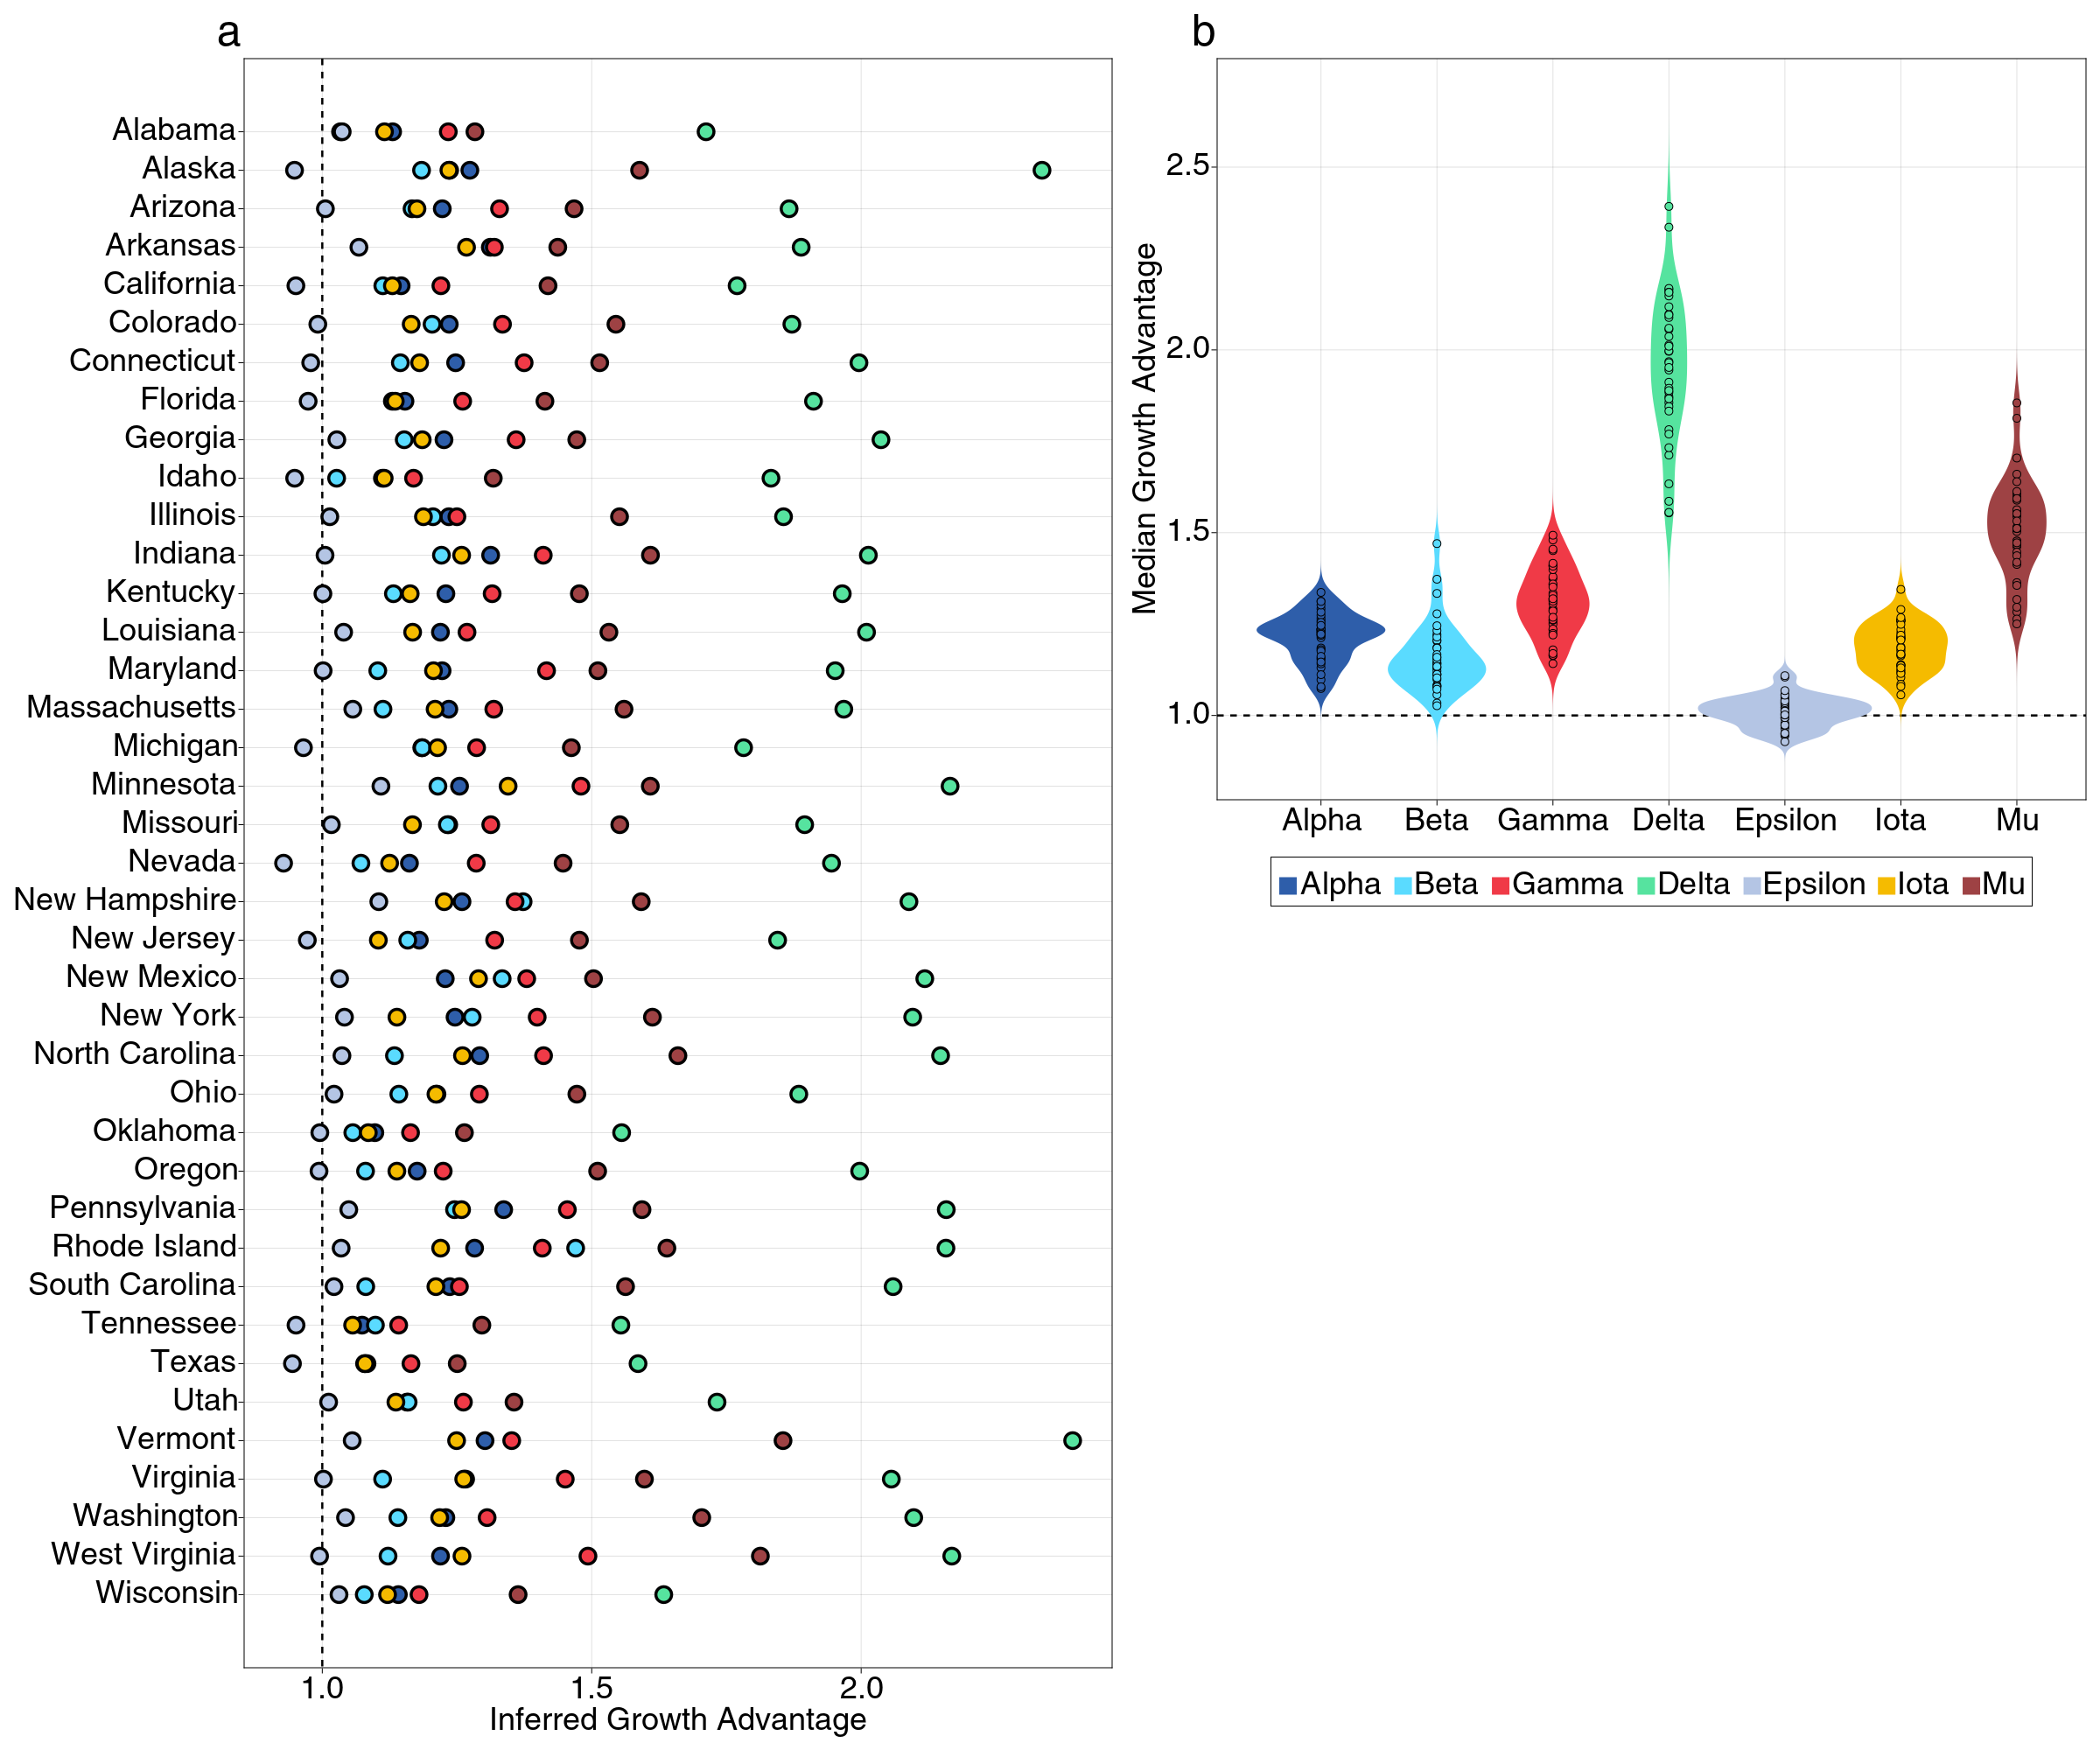
\includegraphics[width=\linewidth]{figs/fig_MLR_growth_advantages_supp.png}
  \caption{Assess growth advantages in various states using Multinomial Logistic Regression model assuming generation time $T_{g} = 5.2$.
  (a) Growth advantages visualized by state.
  (b) Same as (a) but grouped by variant.}%
  \label{fig:MLR_growth_advantages}
\end{figure}

\newpage

\subsubsection*{Relating exponential growth rates to relative effective reproduction numbers}

An important relationship of interest is between the exponential growth rate of an epidemic and its effective reproduction number. In the case of our analysis, we are particularly interested in the ratios of variant-specific effective reproduction numbers. First, notice that the effective reproduction number and the exponential growth rate of an epidemic are related by
\begin{align*}
R_{t} = \frac{1}{\int_{0}^{\infty} \exp(-r\tau)g(\tau)d\tau} = \frac{1}{M_{g}(-r)}
\end{align*}
according to the Lotka-Euler equation \cite{Wallinga2006} where $r$ is the exponential growth rate and $M_{g}$ is the moment-generating function of the generation time $g$.
This allows us to write the relative reproduction number of two variants $v$ and $u$ as a function of their exponential growth rates, so that
\begin{align*}
\frac{R_{t,v}}{R_{t,u}} = \frac{M_{g}(-r_{u})}{M_{g}(-r_{v})}.
\end{align*}

We'll consider three common generation time assumptions. First, we consider the case where the generation time is a point mass at $T_{g}$. In which case, $M_{g}(-r) = \exp(-r T_{g})$ and we recover the relationship
\begin{align*}
\frac{R_{t,v}}{R_{t,u}} = \exp( (r_{v}-r_{u})T_{g}).
\end{align*}

In this case, the relative effective reproduction number depends on only the difference between the exponential growth rates and therefore, is commonly used when converting exponential growth rates to relative reproduction numbers in the case of logistic growth models.

Second, we consider the case where the the generation time is an exponential distribution with mean $T_{g}$. This assumption is often implicit and common in models of infectious diseases such as ODEs and their stochastic variants. Using the corresponding moment-generating function, we see that
\begin{align*}
\frac{R_{t,v}}{R_{t,u}} = \frac{1 + r_{v} T_{g}}{1 + r_{u} T_{g}}.
\end{align*}


Next, we consider the Gamma distributed generation times with mean $T_{g}$ and standard deviation $s$. This is often used in models of infectious diseases via the chain trick in which multiple compartments are chained together to obtain non-exponential generation or waiting times. Re-parameterizing the Gamma distribution in terms of its mean and standard deviation, we have that
\begin{align*}
\frac{R_{t,v}}{R_{t,u}} = \left( \frac{1 + r_{v}  \left(\frac{s^{2}}{T_{g}}\right)}{1 + r_{u} \left(\frac{s^{2}}{T_{g}}\right) } \right)^{T_{g}^{2} / s^{2}}.
\end{align*}

From this equation, we can see that increases in the mean of the generation time lead to higher inferred variant advantages given the same growth rates. On the other hand, increases in the standard deviation lead to lower inferred variant advantages. This effect is also visualized in Figure \ref{fig:generation_time_sensitivity}.

Taking a logarithm, we can also evaluate the sensitivity of our inferred growth advantages from our fixed growth advantage model with respect to the generation time assuming it is Gamma distributed as
\begin{align*}
 \delta_{v}  = \ln \left( \frac{R_{t,v}}{R_{t,0}} \right) = \left( \frac{T_{g}^{2}}{s^{2}} \right)  \ln \left( \frac{1 + r_{v}  \left(\frac{s^{2}}{T_{g}}\right)}{1 + r_{0} \left(\frac{s^{2}}{T_{g}}\right) } \right).
\end{align*}
The behavior here is analogous to that discussed above when the mean $T_{g}$ and standard deviation $s$ are changed although these growth advantages appear to relatively stable under varying standard deviation in Figure \ref{fig:growth_advantage_sensitivity}.

The cases of exponential and Gamma-distributed generation times highlight that for non-deterministic generation times there is no guarantee that the relative effective reproduction number depends on only the difference in exponential growth rates.
In fact, these estimates based on the deterministic generation times correspond to the case in which the standard deviation shrinks zero, they are likely overestimates of variant advantages given the observed variation in the serial interval of SARS-CoV-2 infections.

\begin{figure}
  \centering
  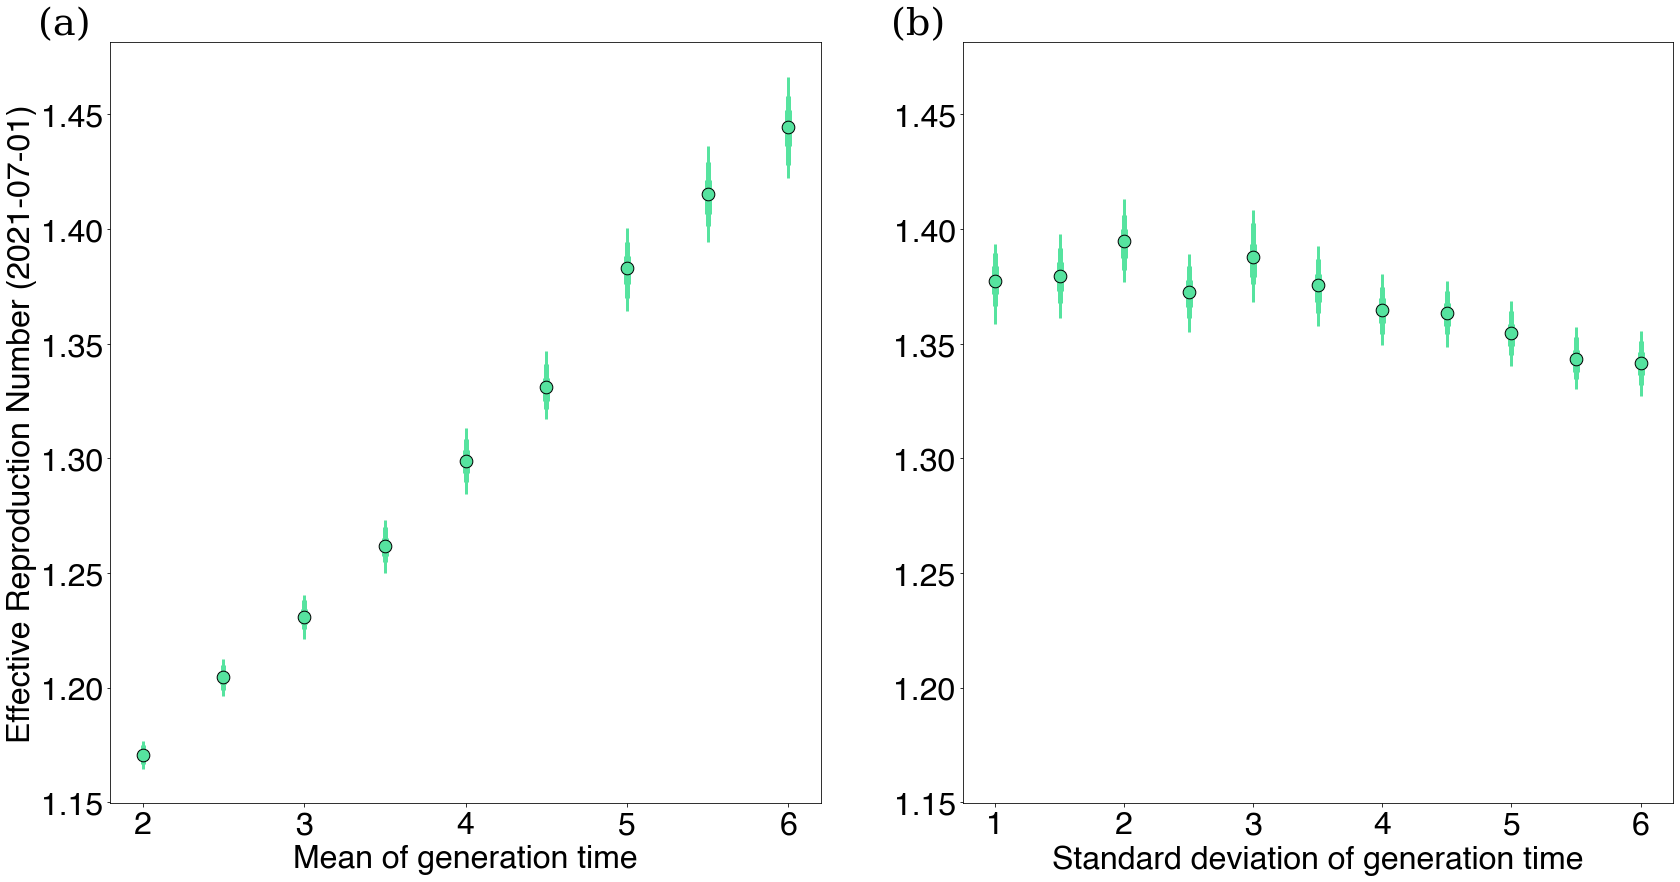
\includegraphics[width=\linewidth]{figs/generation_time_sensitivity.png}
  \caption{\textbf{Sensitivity of effective reproduction number to changes in generation time.} (a) We vary the mean of the generation time keeping a constant standard deviation 1.72 and plot against effective reproduction number estimates for Delta in Washington state on July 1st, 2021 using our free $R_{t}$ model.  (b) The same as (a), but we instead vary the standard deviation of the generation time keeping a constant mean 5.2.}%
  \label{fig:generation_time_sensitivity}
\end{figure}

\begin{figure}
  \centering
  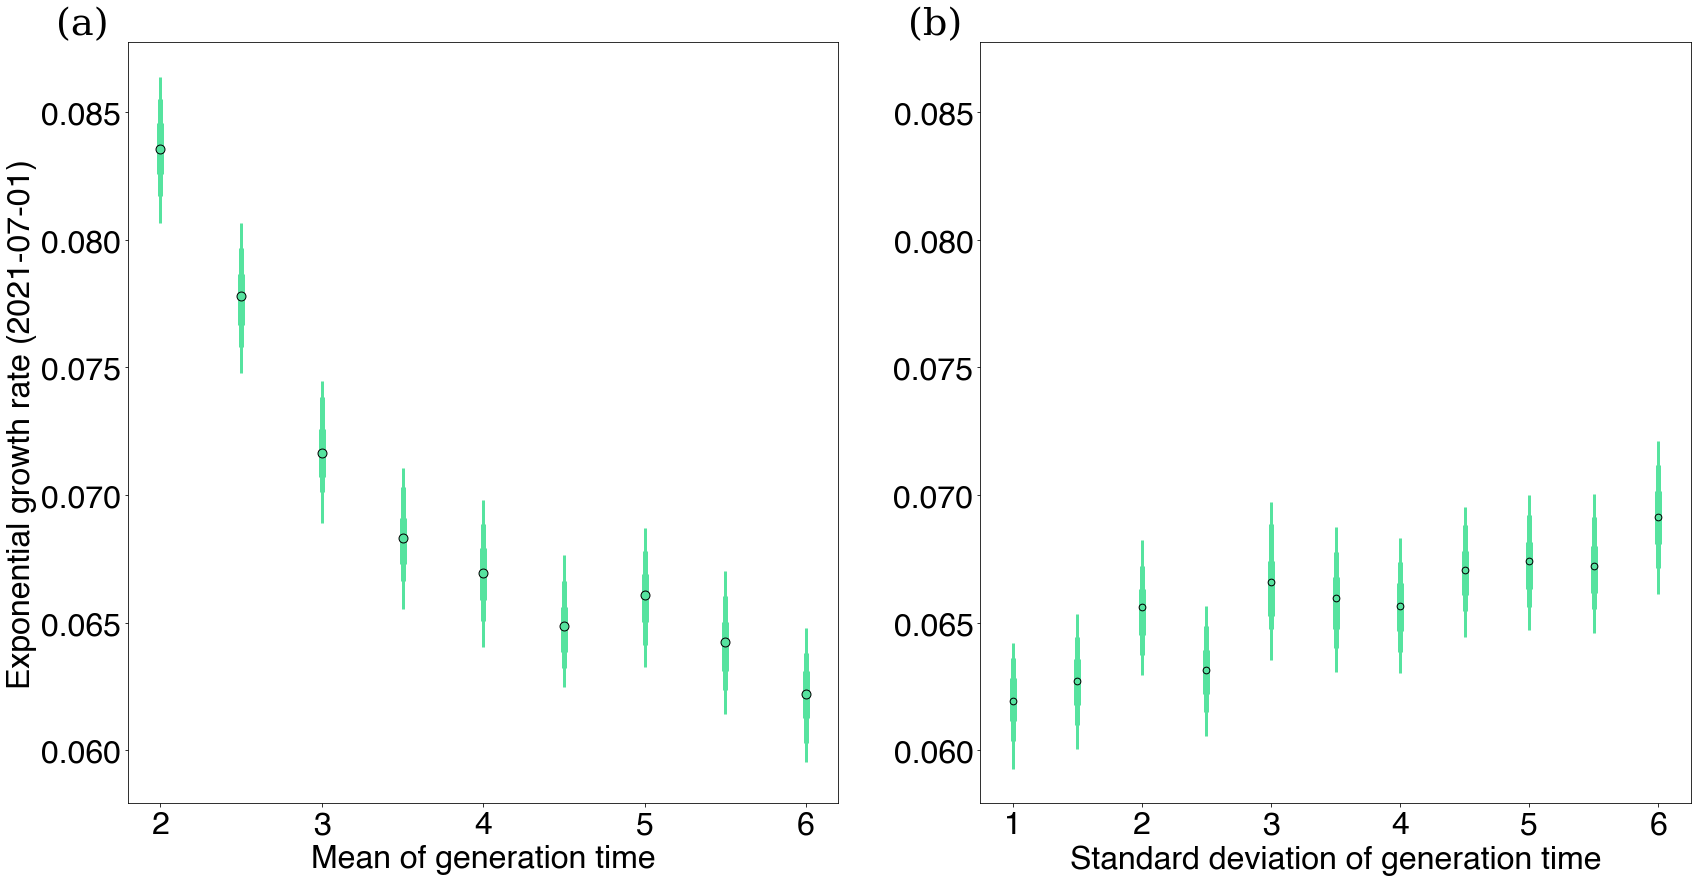
\includegraphics[width=\linewidth]{figs/little_r_sensitivity.png}
  \caption{\textbf{Sensitivity of exponential growth rates to changes in generation time.} (a) We vary the mean of the generation time keeping a constant standard deviation 1.72 and plot against exponential growth rates for Delta in Washington state on July 1st, 2021 using our free $R_{t}$ model and assuming a Gamma-distributed generation time.  (b) The same as (a), but we instead vary the standard deviation of the generation time keeping a constant mean 5.2. }%
  \label{fig:little_r_sensitivity}
\end{figure}

\begin{figure}
  \centering
  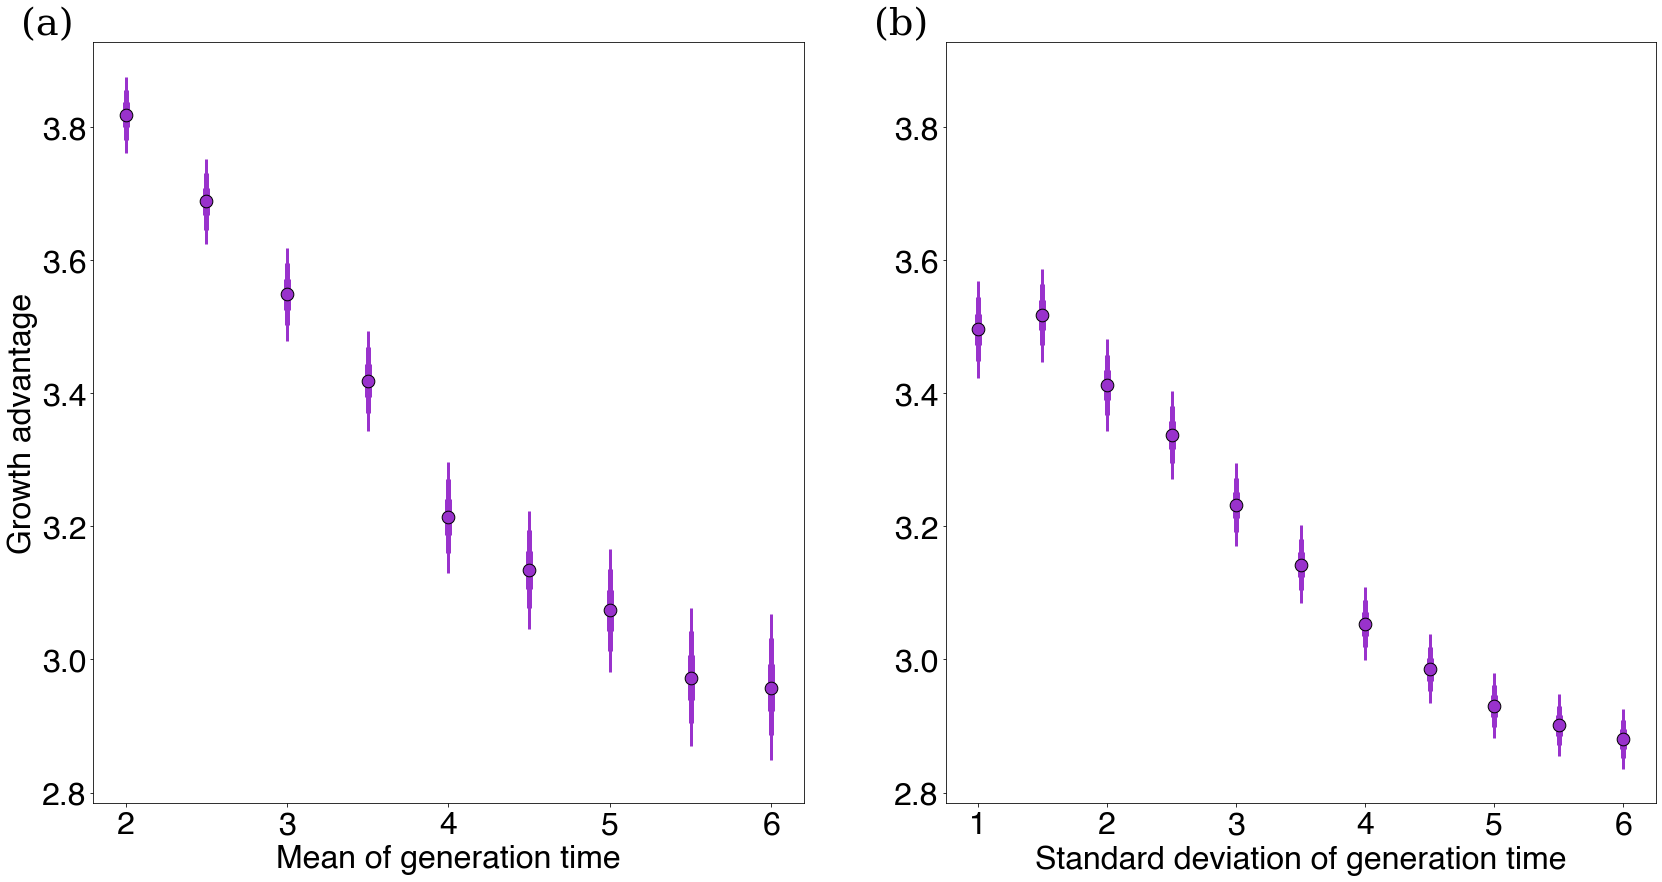
\includegraphics[width=\linewidth]{figs/growth_advantage_sensitivity.png}
  \caption{\textbf{Sensitivity of growth advantages to changes in generation time.} (a) We vary the mean of the generation time keeping a constant standard deviation 1.72 and plot against exponential growth rates for Delta in Washington state on July 1st, 2021 using our fixed growth model.  (b) The same as (a), but we instead vary the standard deviation of the generation time keeping a constant mean 5.2.}%
  \label{fig:growth_advantage_sensitivity}
\end{figure}


\begin{figure}
  \centering
  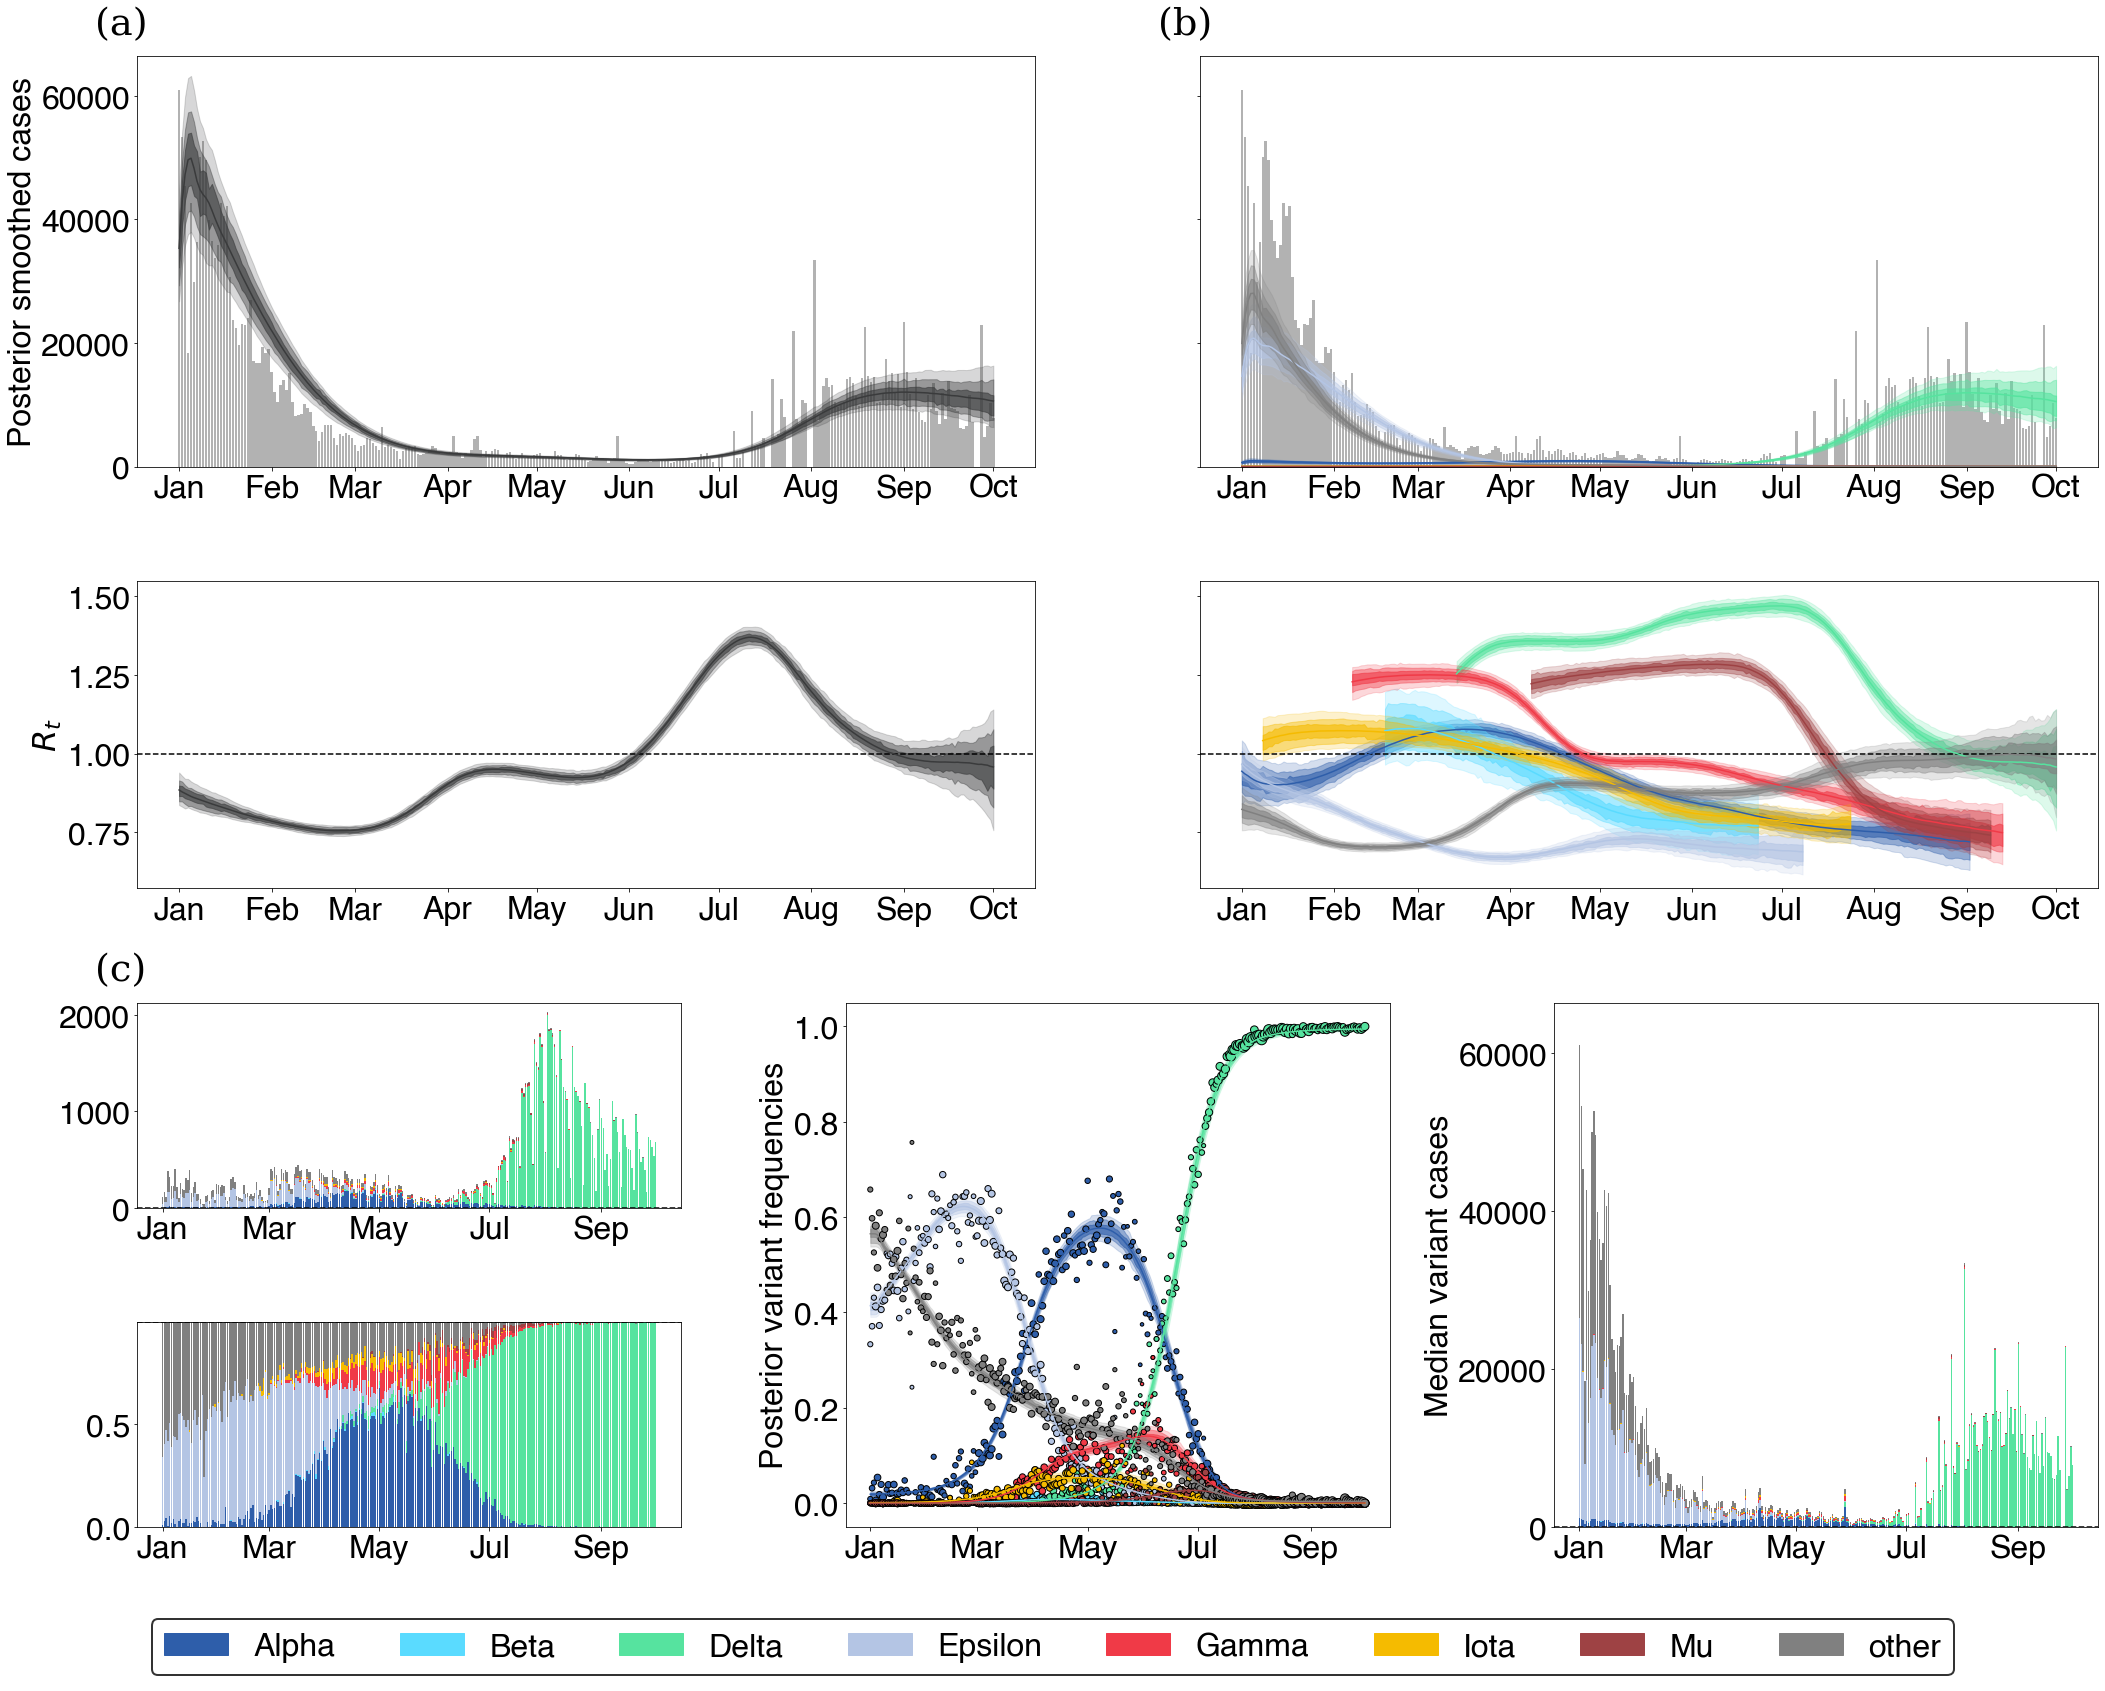
\includegraphics[width=\linewidth]{figs/free_rt_California.png}
  \caption{\textbf{Fitting the free $R_{t}$ model to California data.}}%
  \label{fig:free_rt_California}
\end{figure}

\begin{figure}
  \centering
  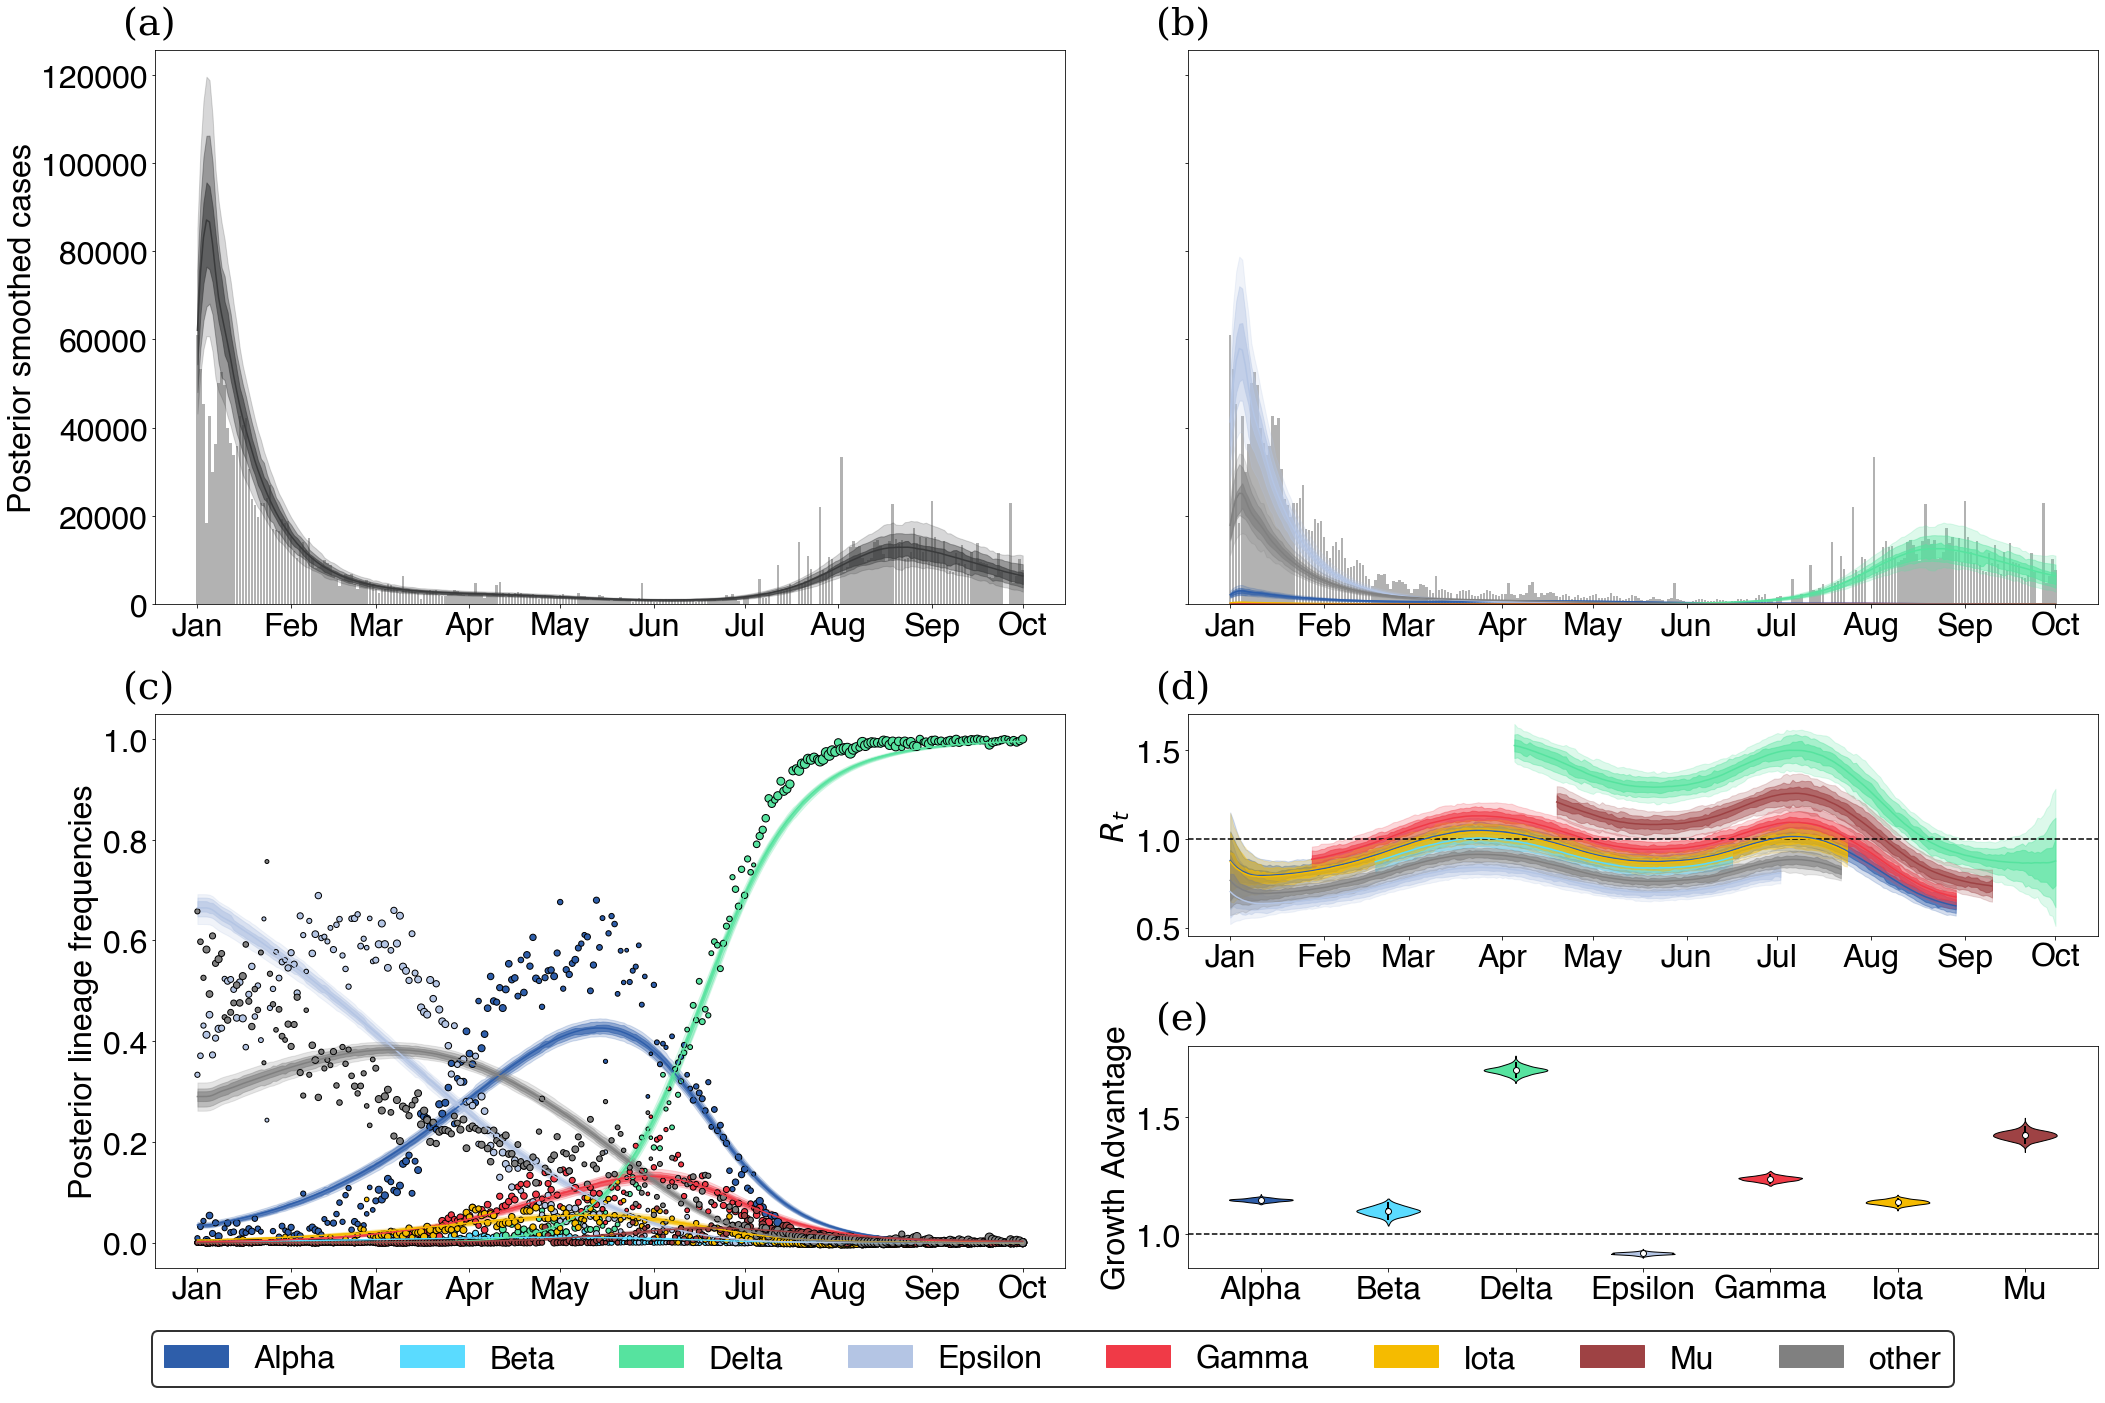
\includegraphics[width=\linewidth]{figs/fixed_growth_California.png}
  \caption{\textbf{Fitting the fixed growth advantage model to California data.}}%
  \label{fig:fixed_growth_California}
\end{figure}

\begin{figure}
  \centering
  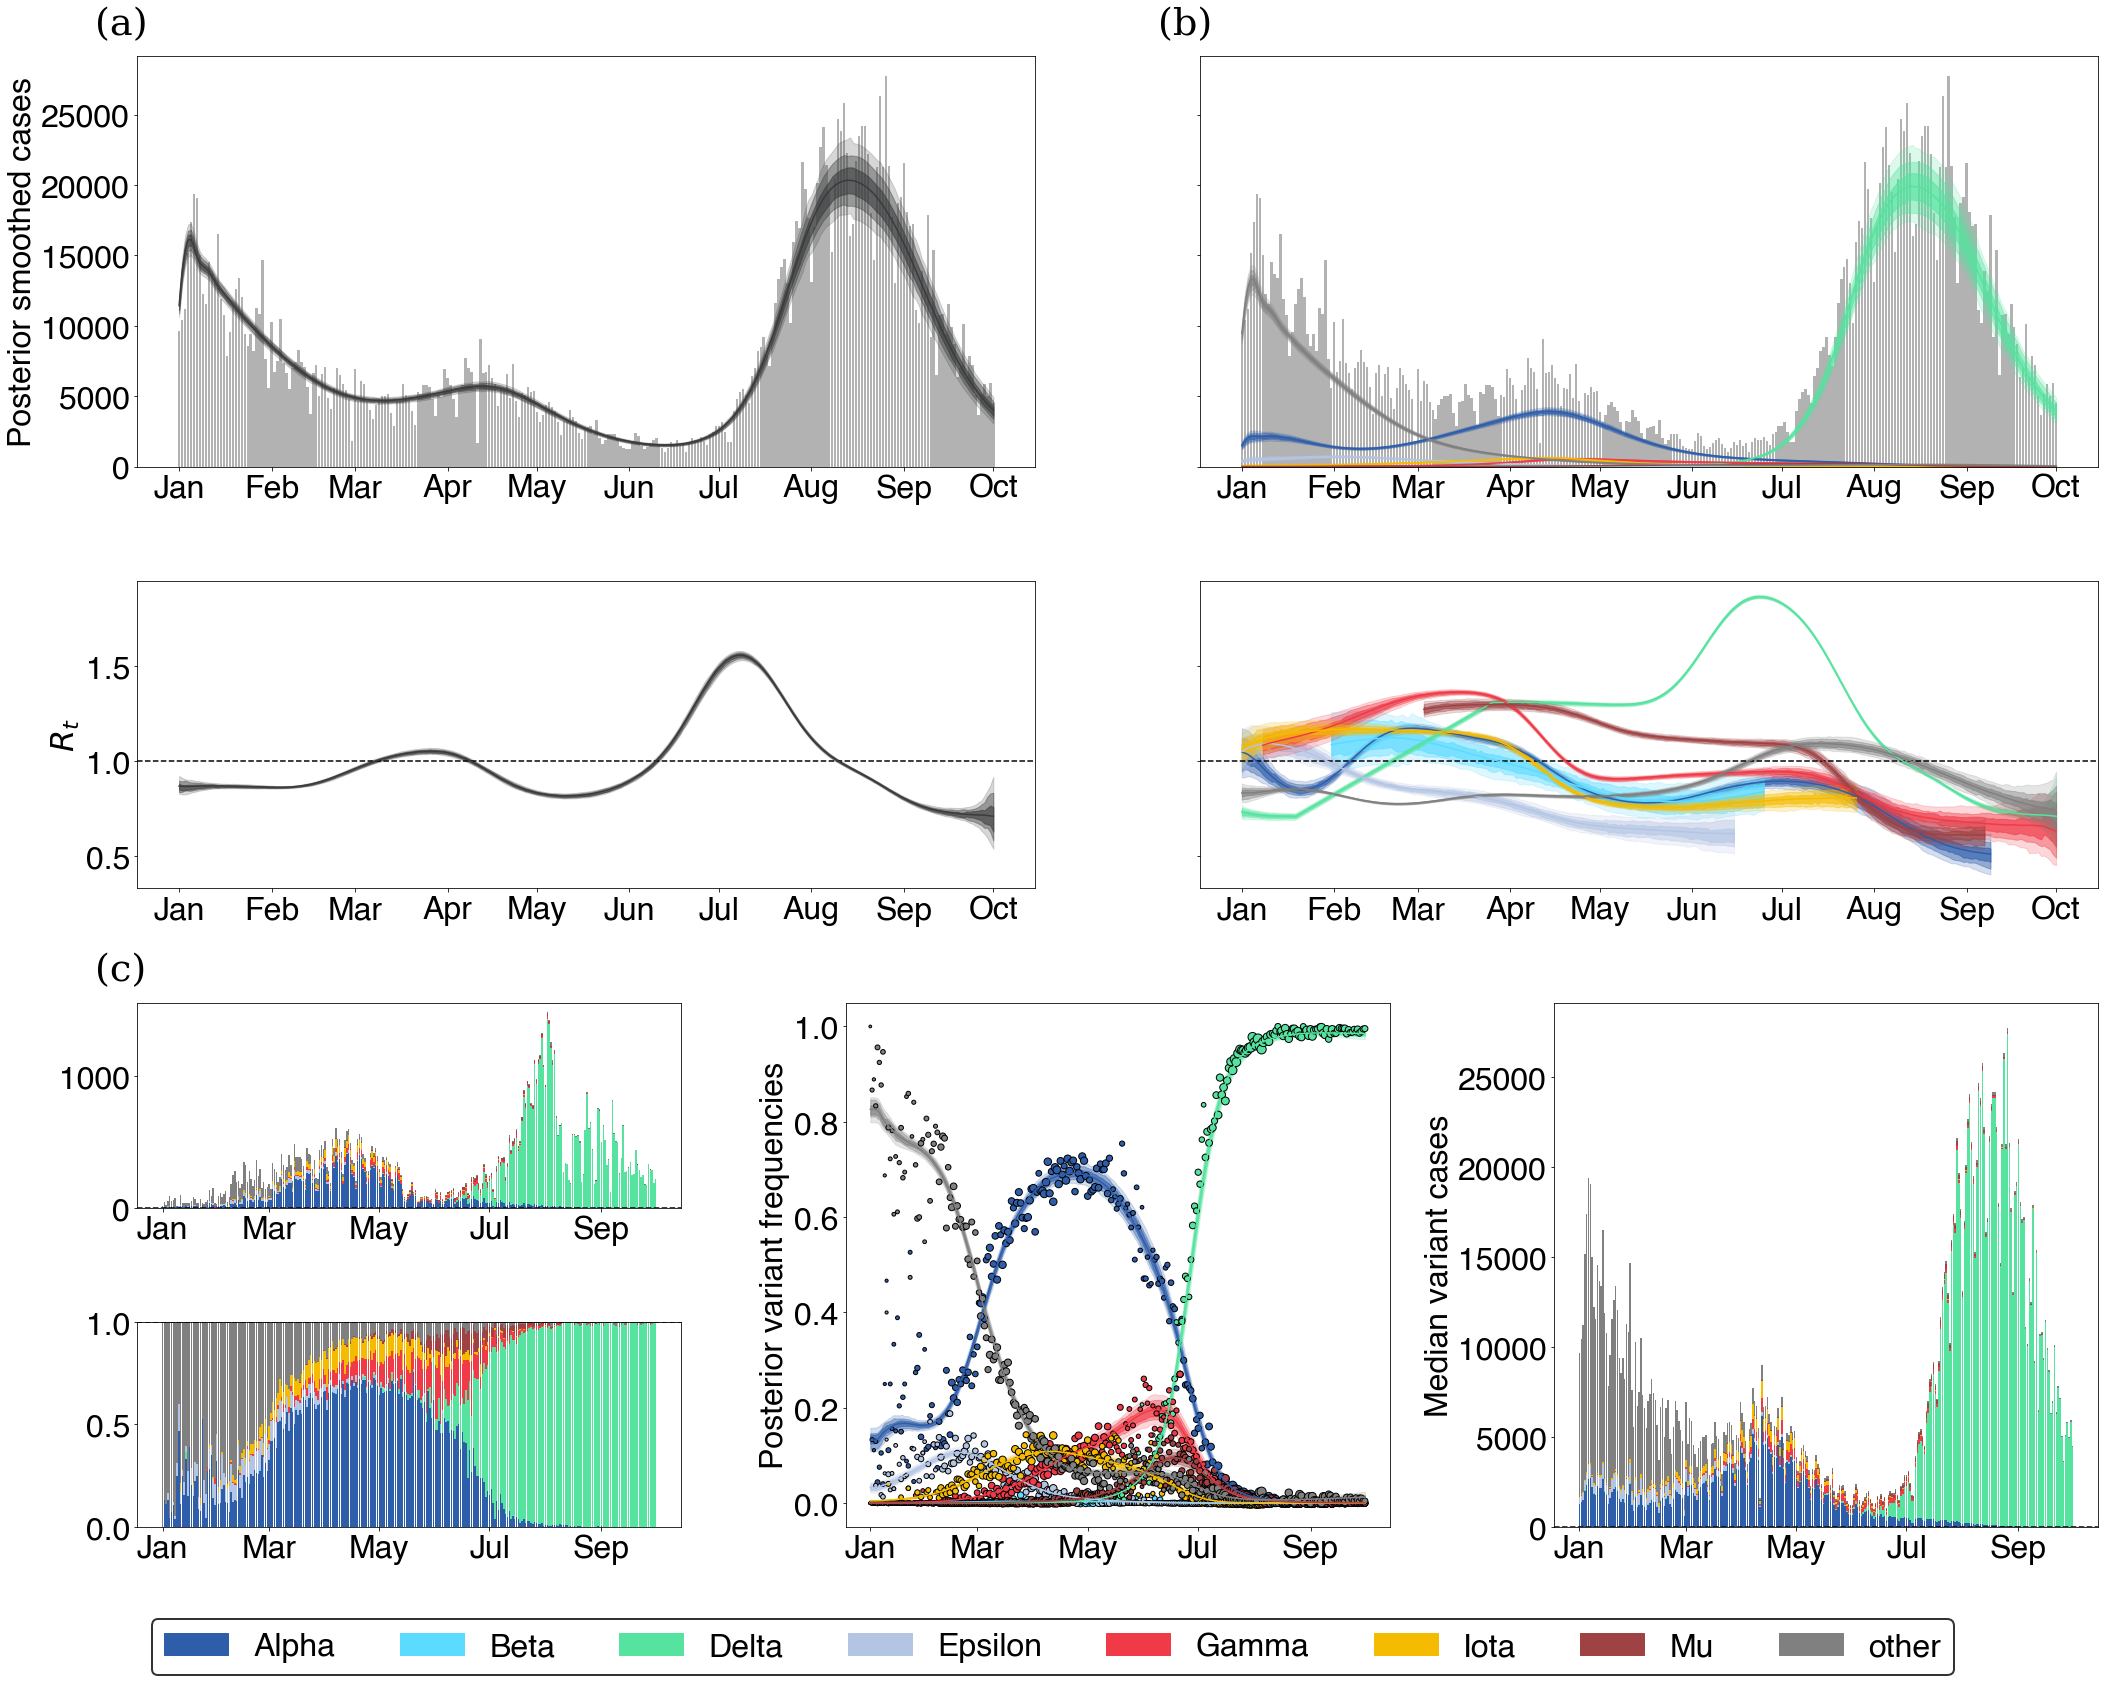
\includegraphics[width=\linewidth]{figs/free_rt_Florida.png}
  \caption{\textbf{Fitting the free $R_{t}$ model to Florida data.}}%
  \label{fig:free_rt_Florida}
\end{figure}

\begin{figure}
  \centering
  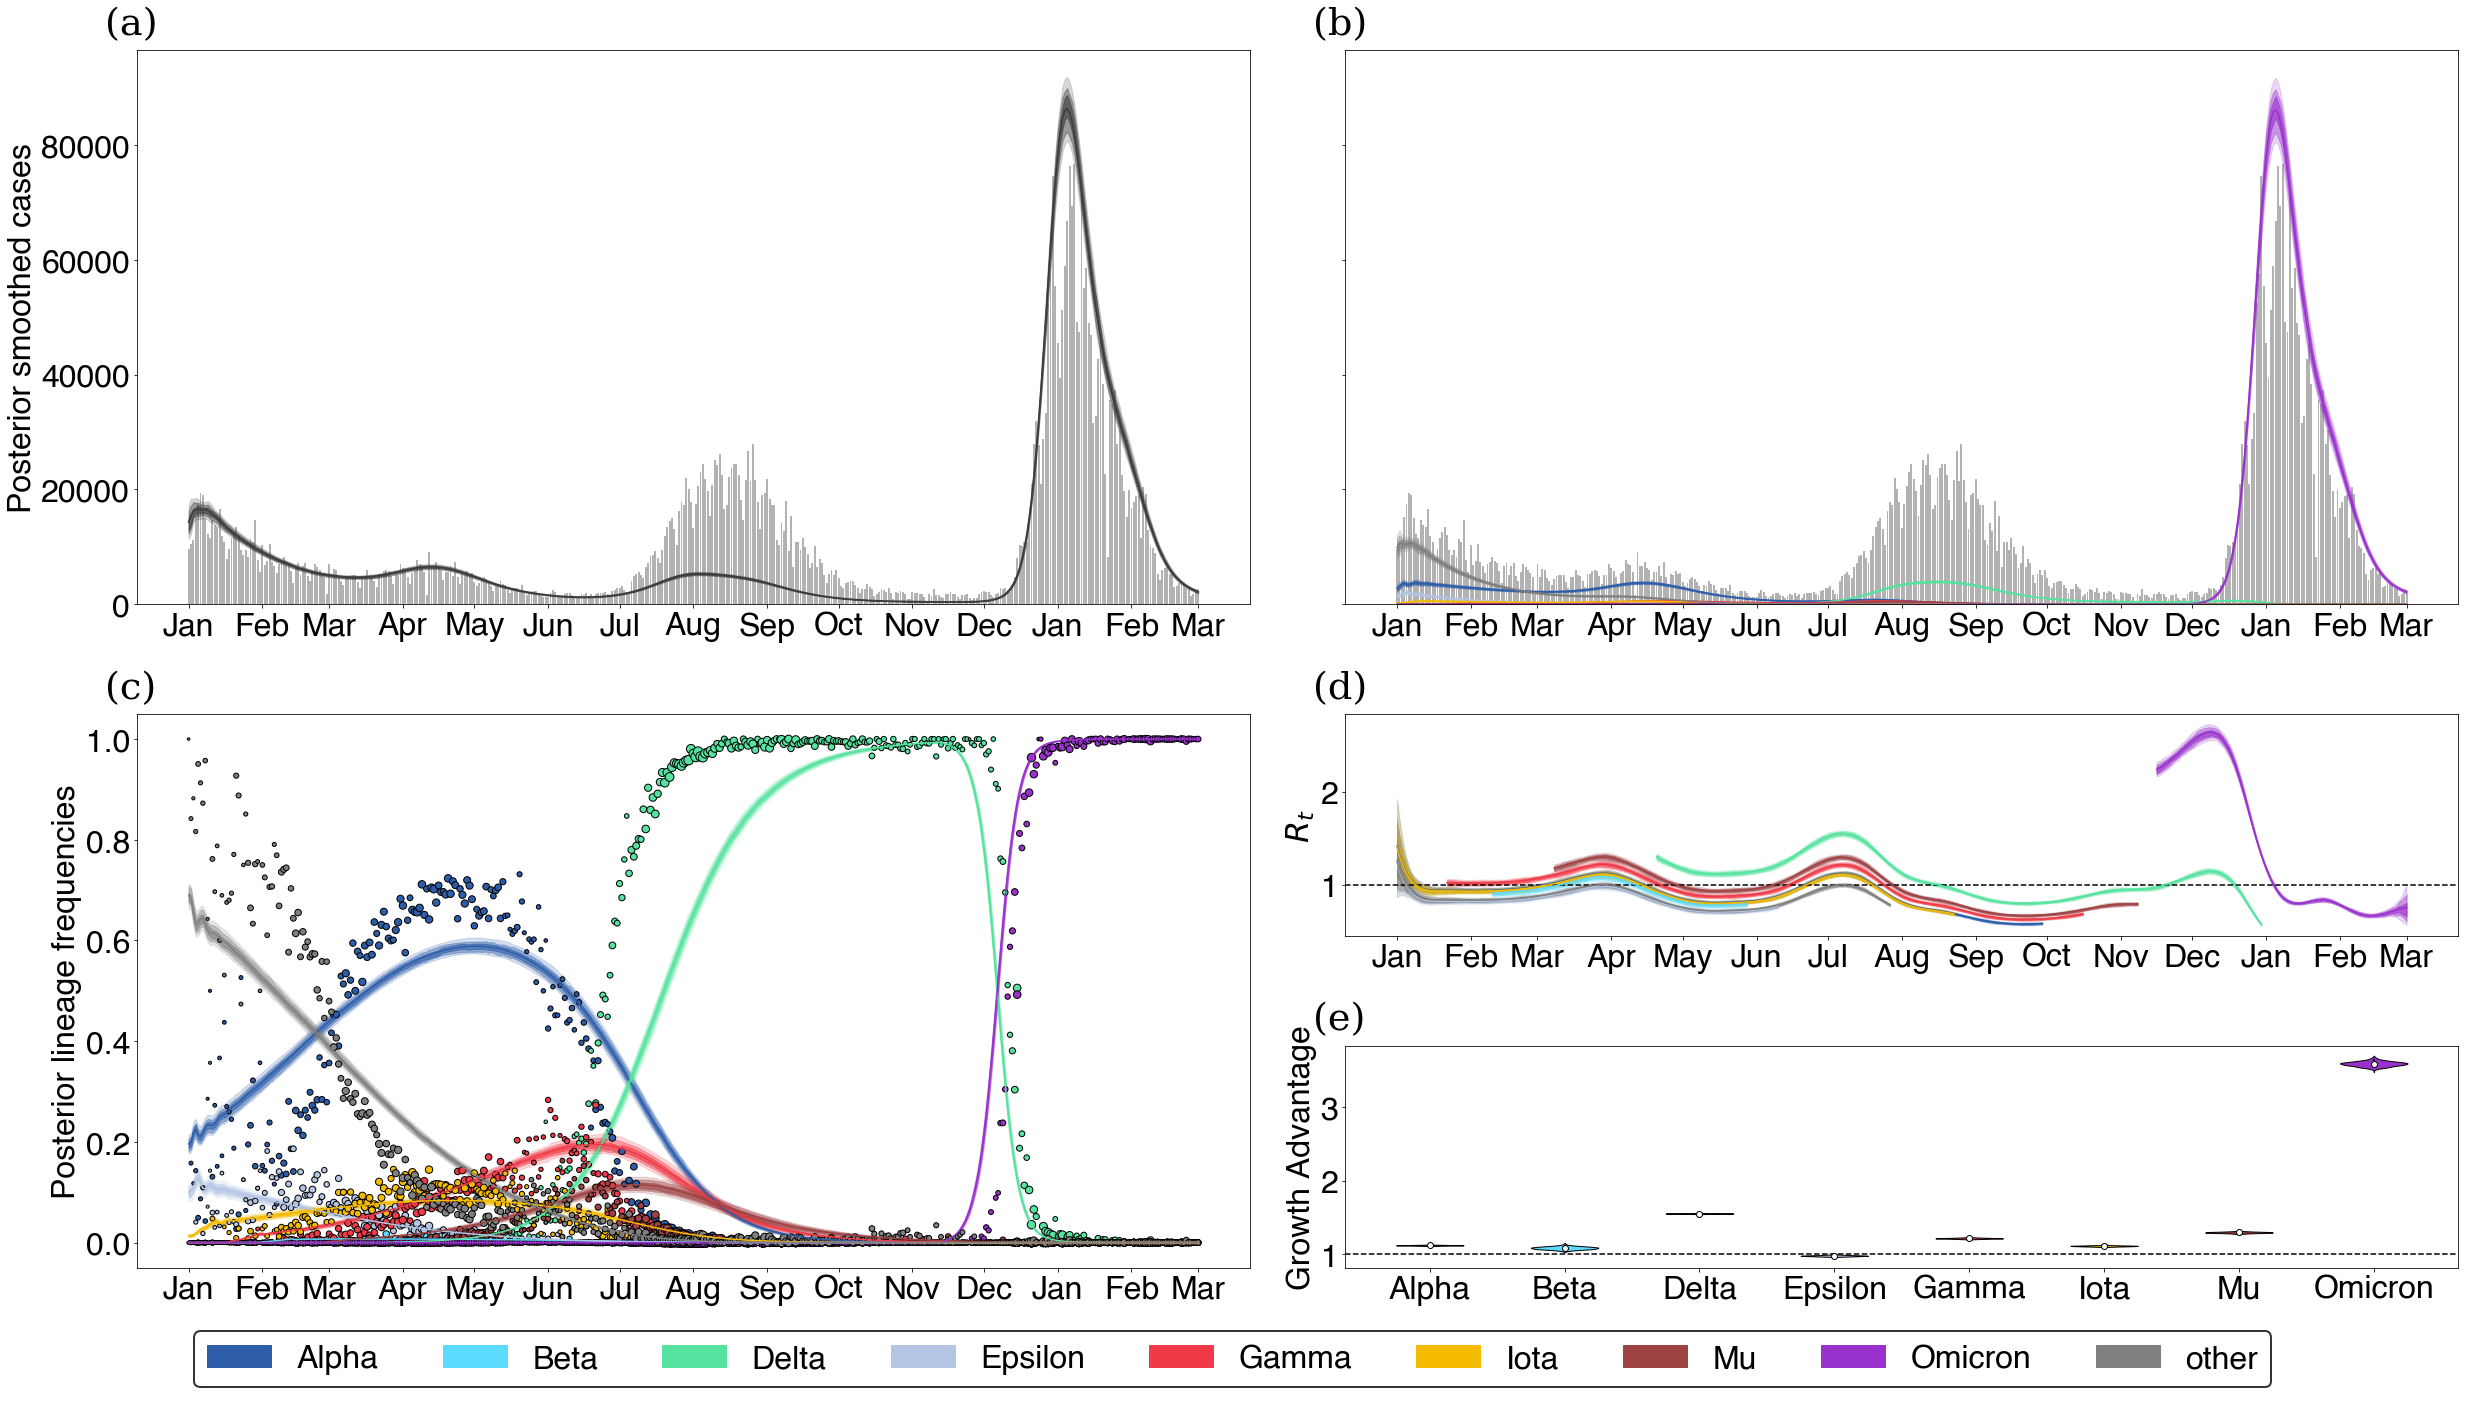
\includegraphics[width=\linewidth]{figs/fixed_growth_Florida.png}
  \caption{\textbf{Fitting the fixed growth advantage model to Florida data.}}%
  \label{fig:fixed_growth_Florida}
\end{figure}

\begin{figure}
  \centering
  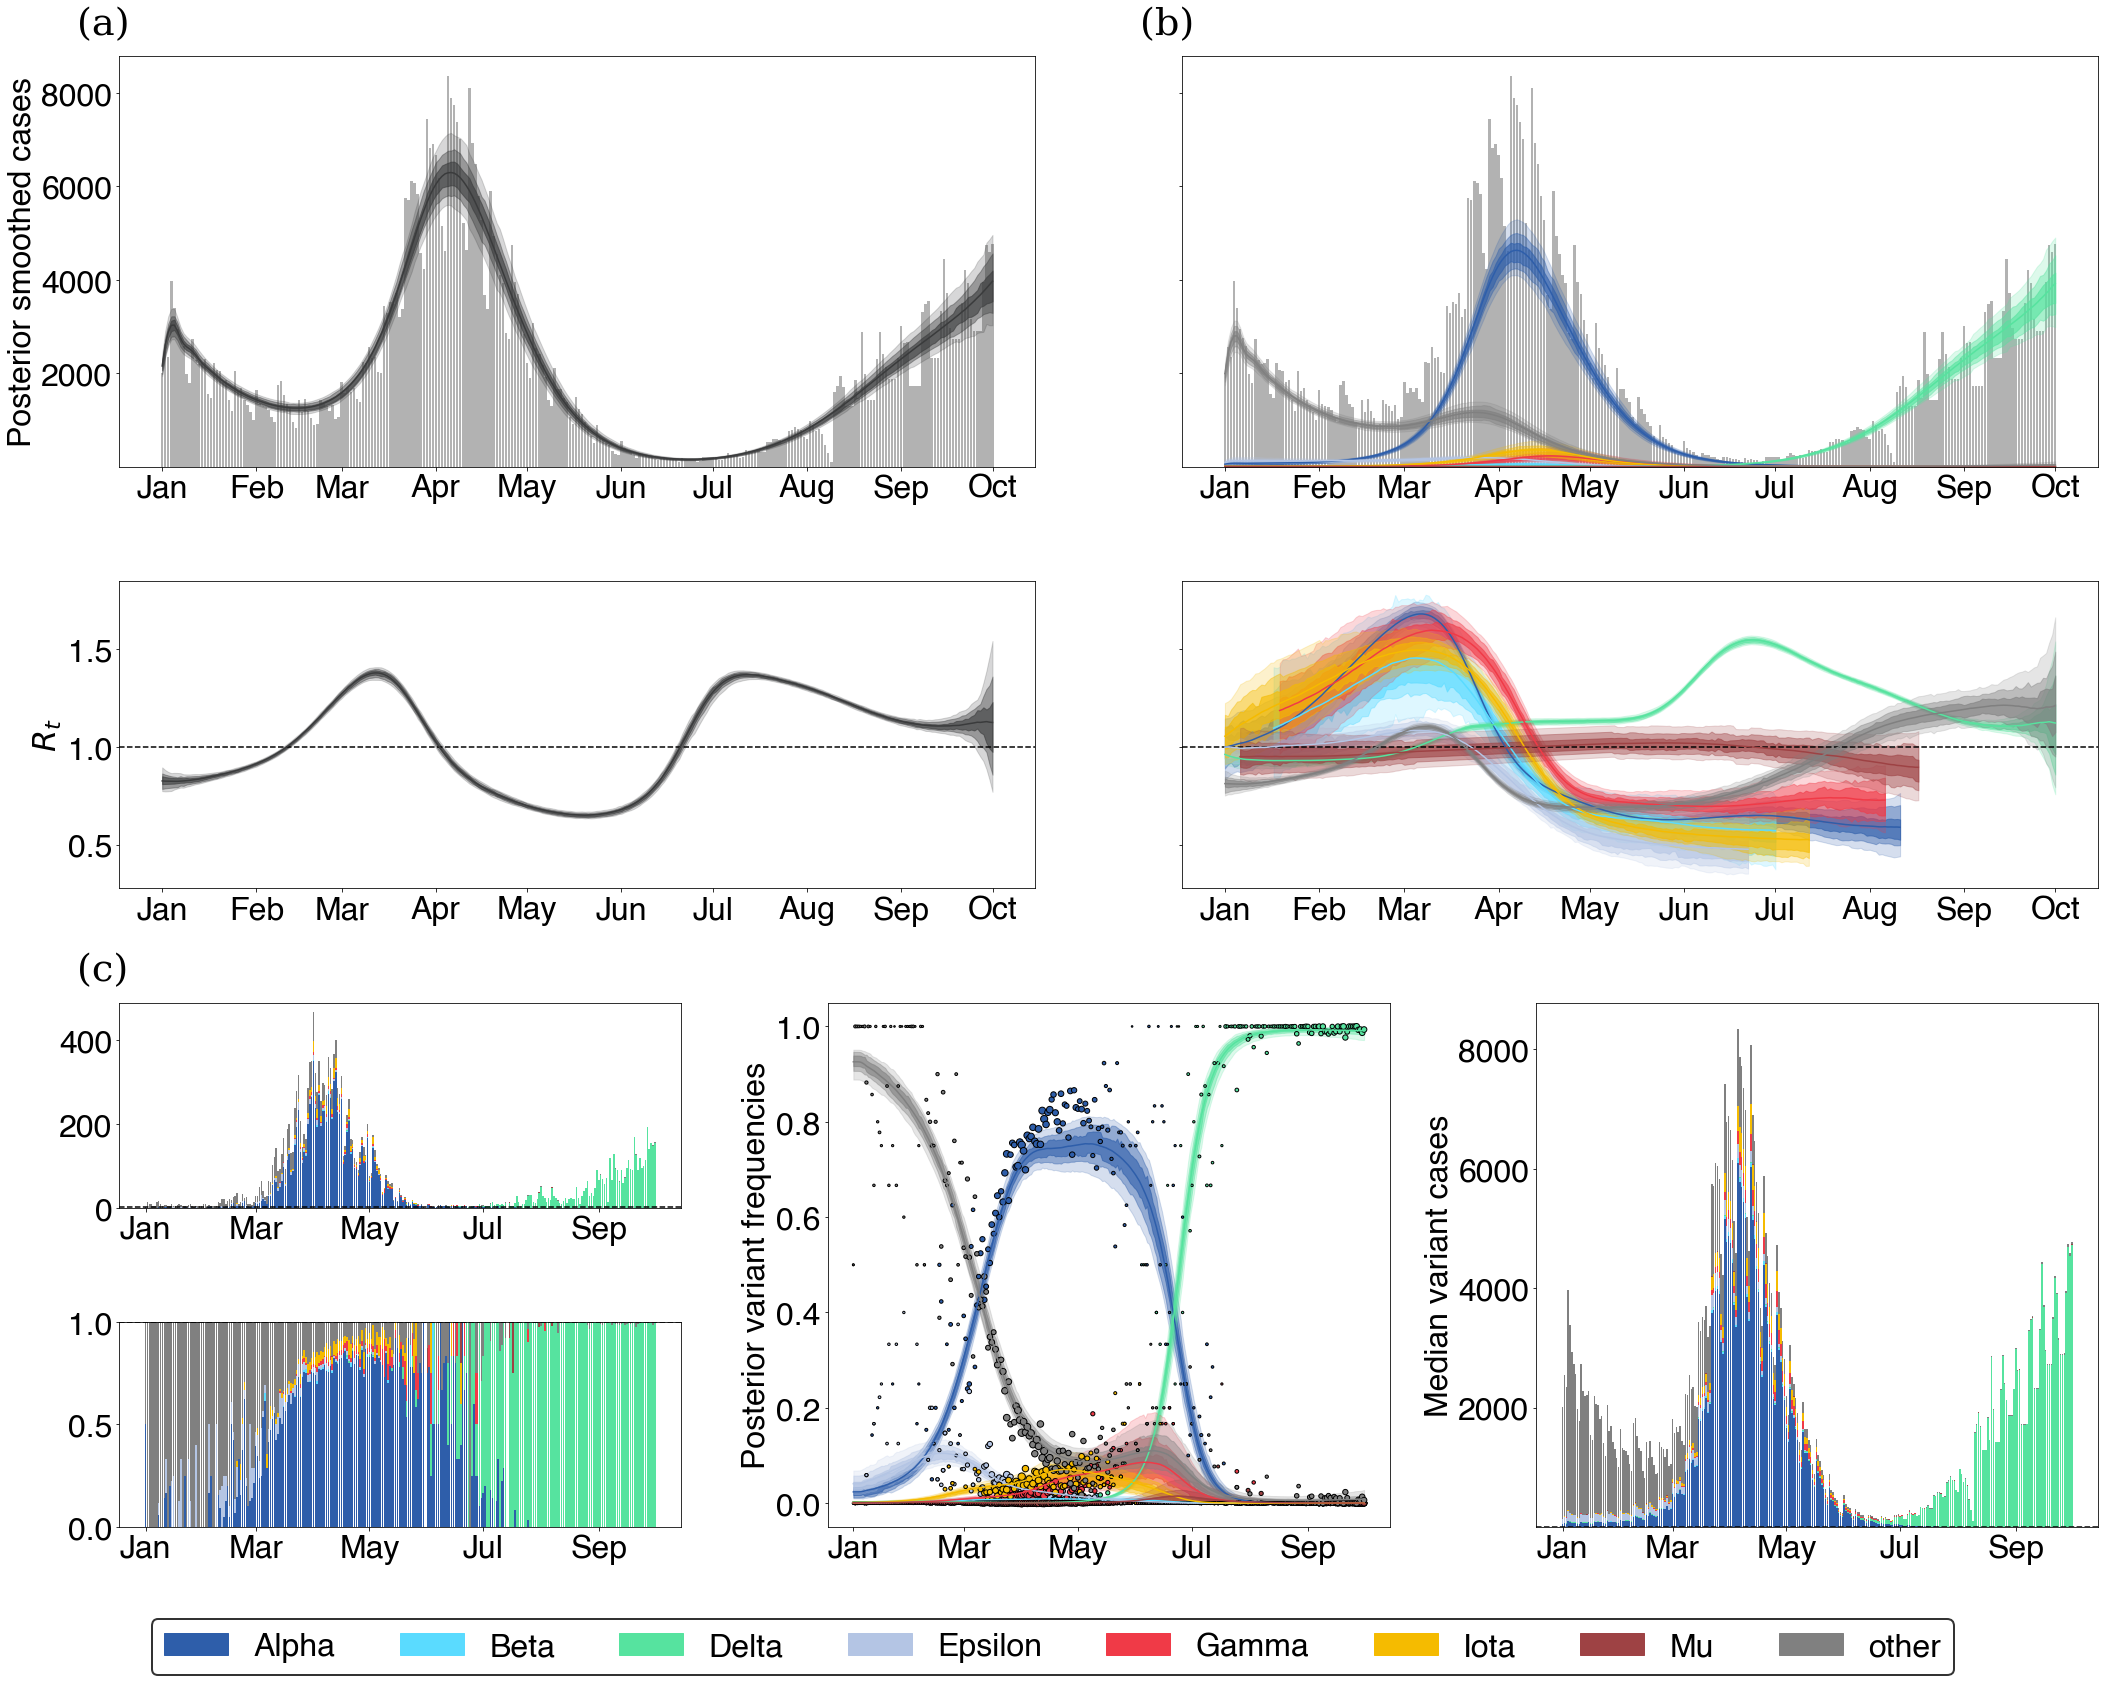
\includegraphics[width=\linewidth]{figs/free_rt_Michigan.png}
  \caption{\textbf{Fitting the free $R_{t}$ model to Michigan data.}}%
  \label{fig:free_rt_Michigan}
\end{figure}

\begin{figure}
  \centering
  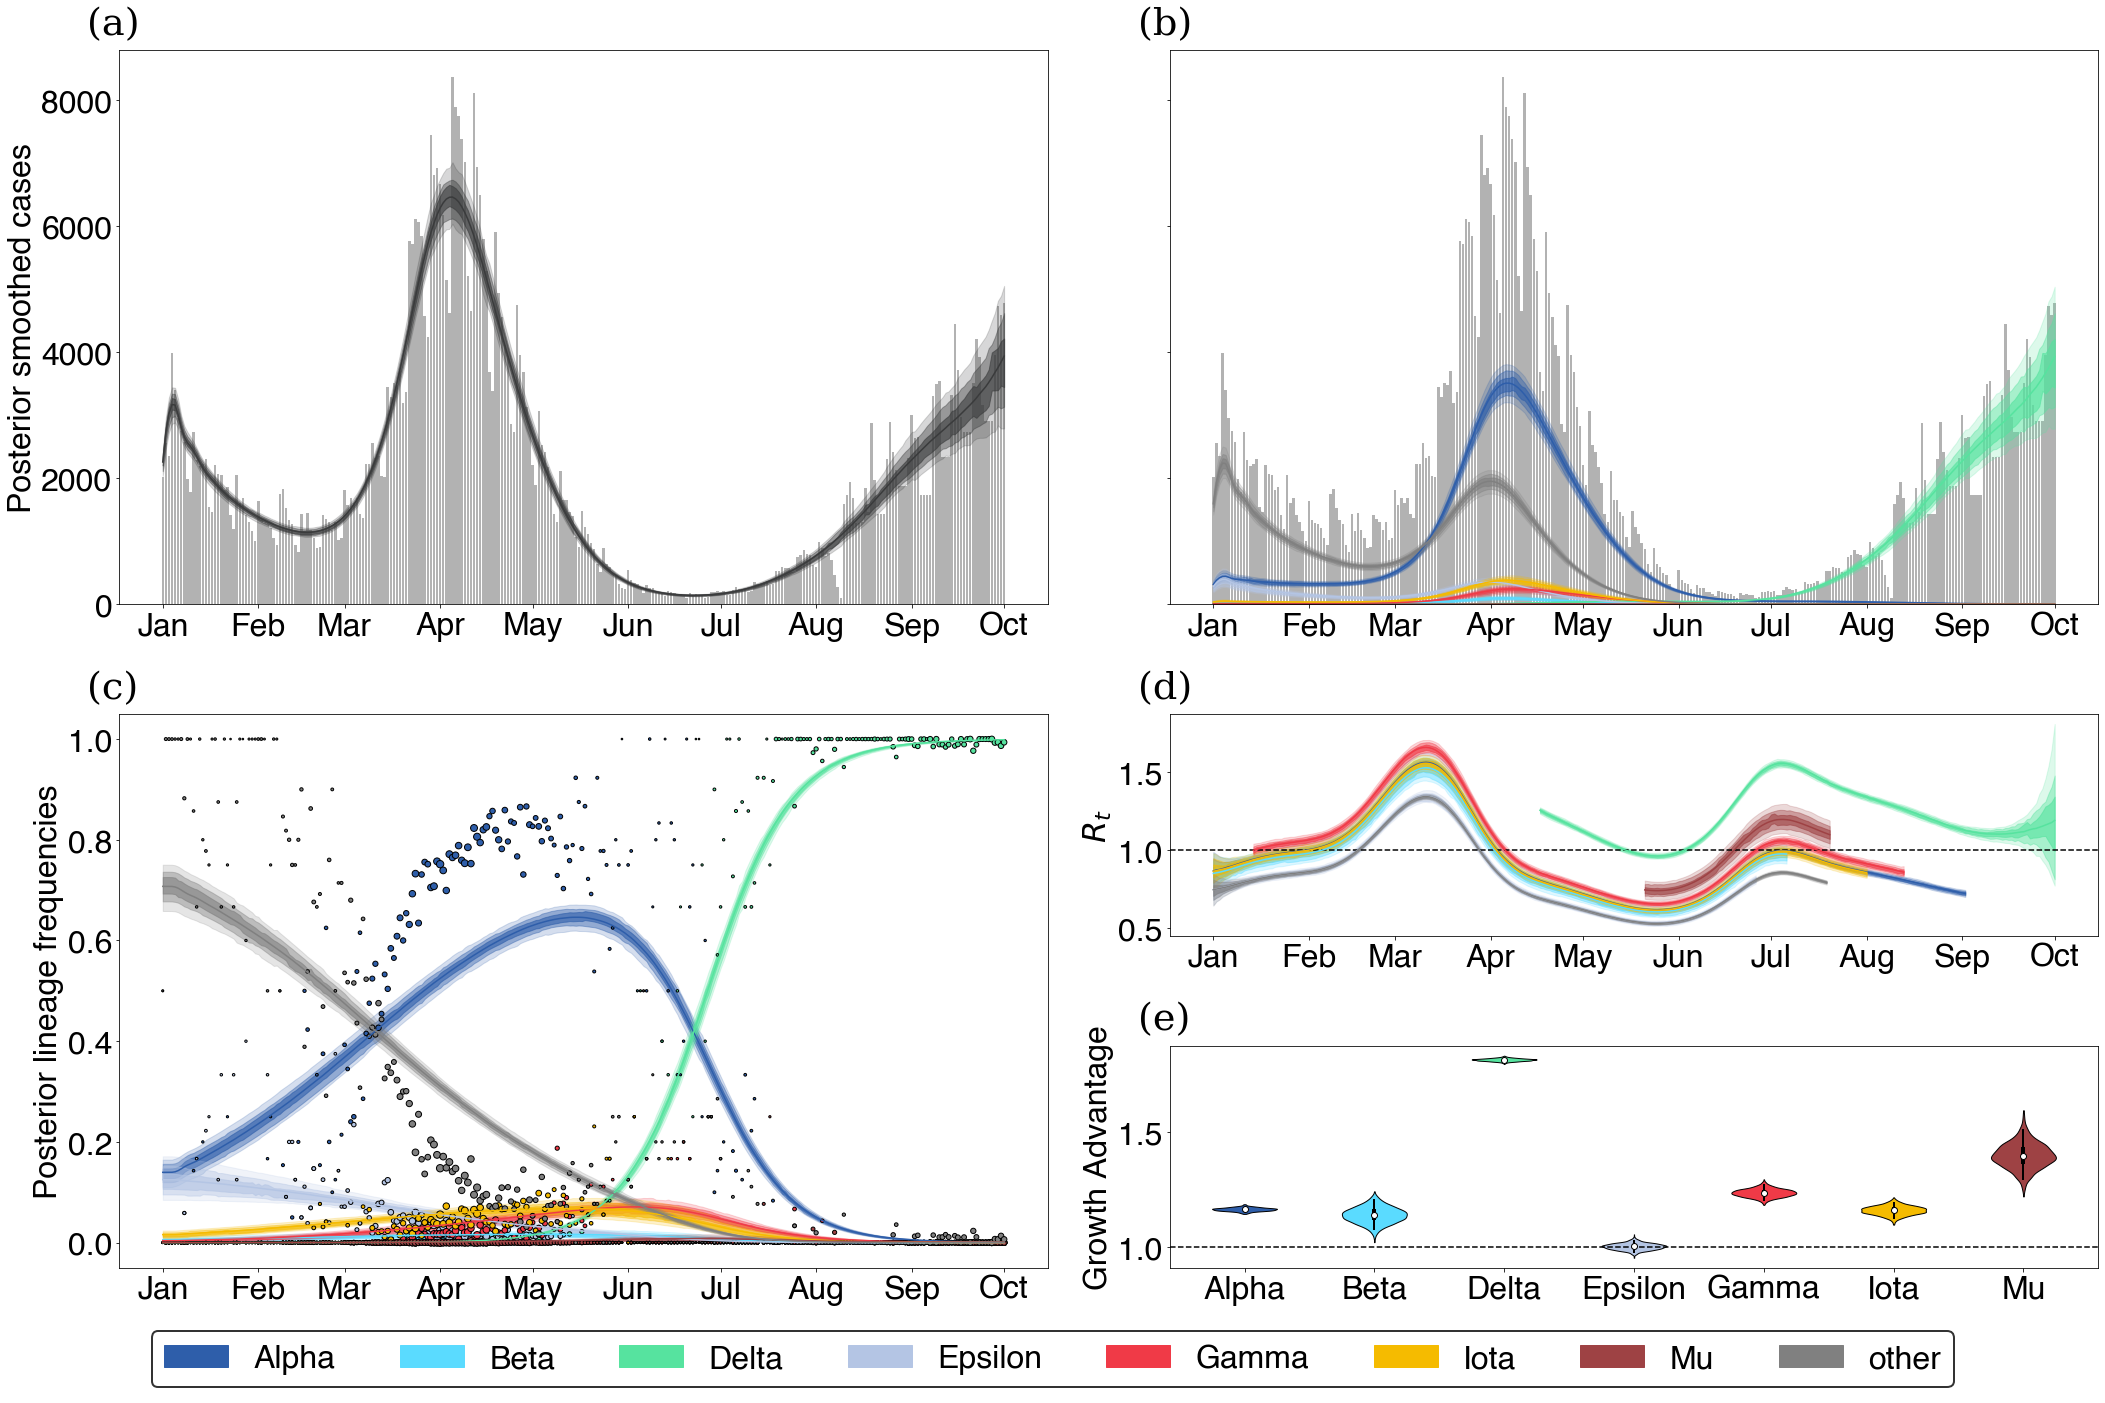
\includegraphics[width=\linewidth]{figs/fixed_growth_Michigan.png}
  \caption{\textbf{Fitting the fixed growth advantage model to Michigan data.}}%
  \label{fig:fixed_growth_Michigan}
\end{figure}


\begin{figure}
  \centering
  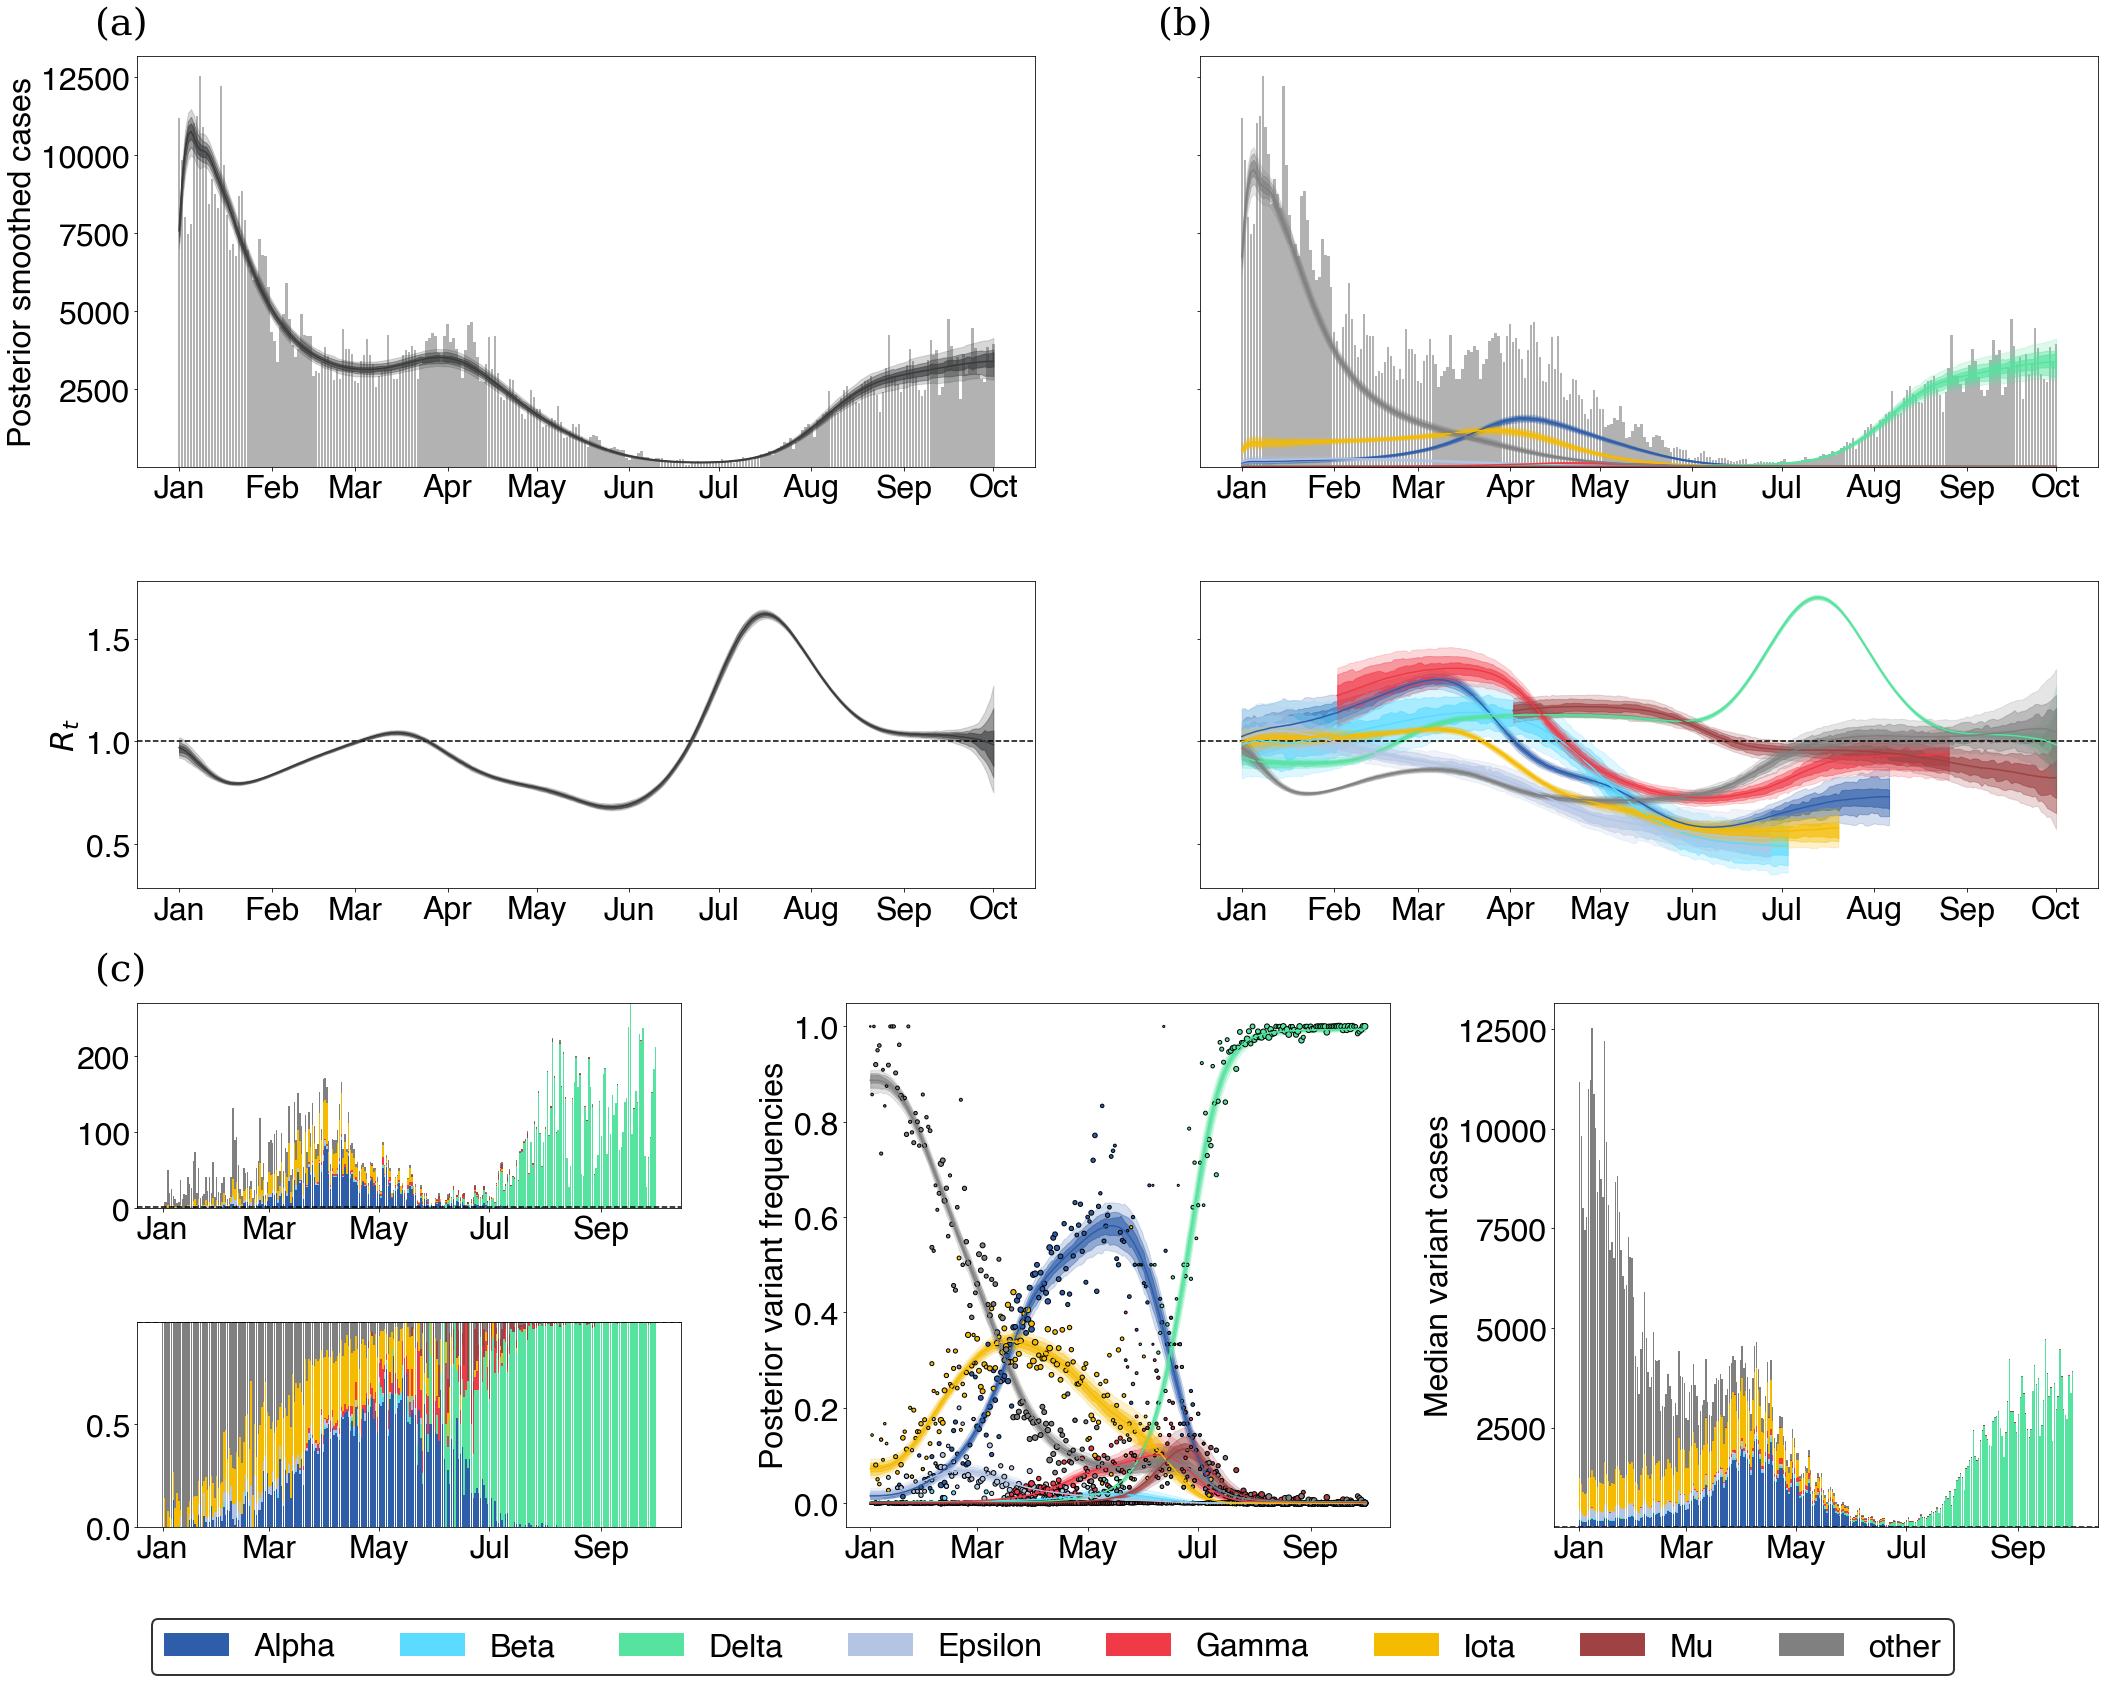
\includegraphics[width=\linewidth]{figs/free_rt_New-York.png}
  \caption{\textbf{Fitting the free $R_{t}$ model to New York state data.}}%
  \label{fig:free_rt_New-York}
\end{figure}

\begin{figure}
  \centering
  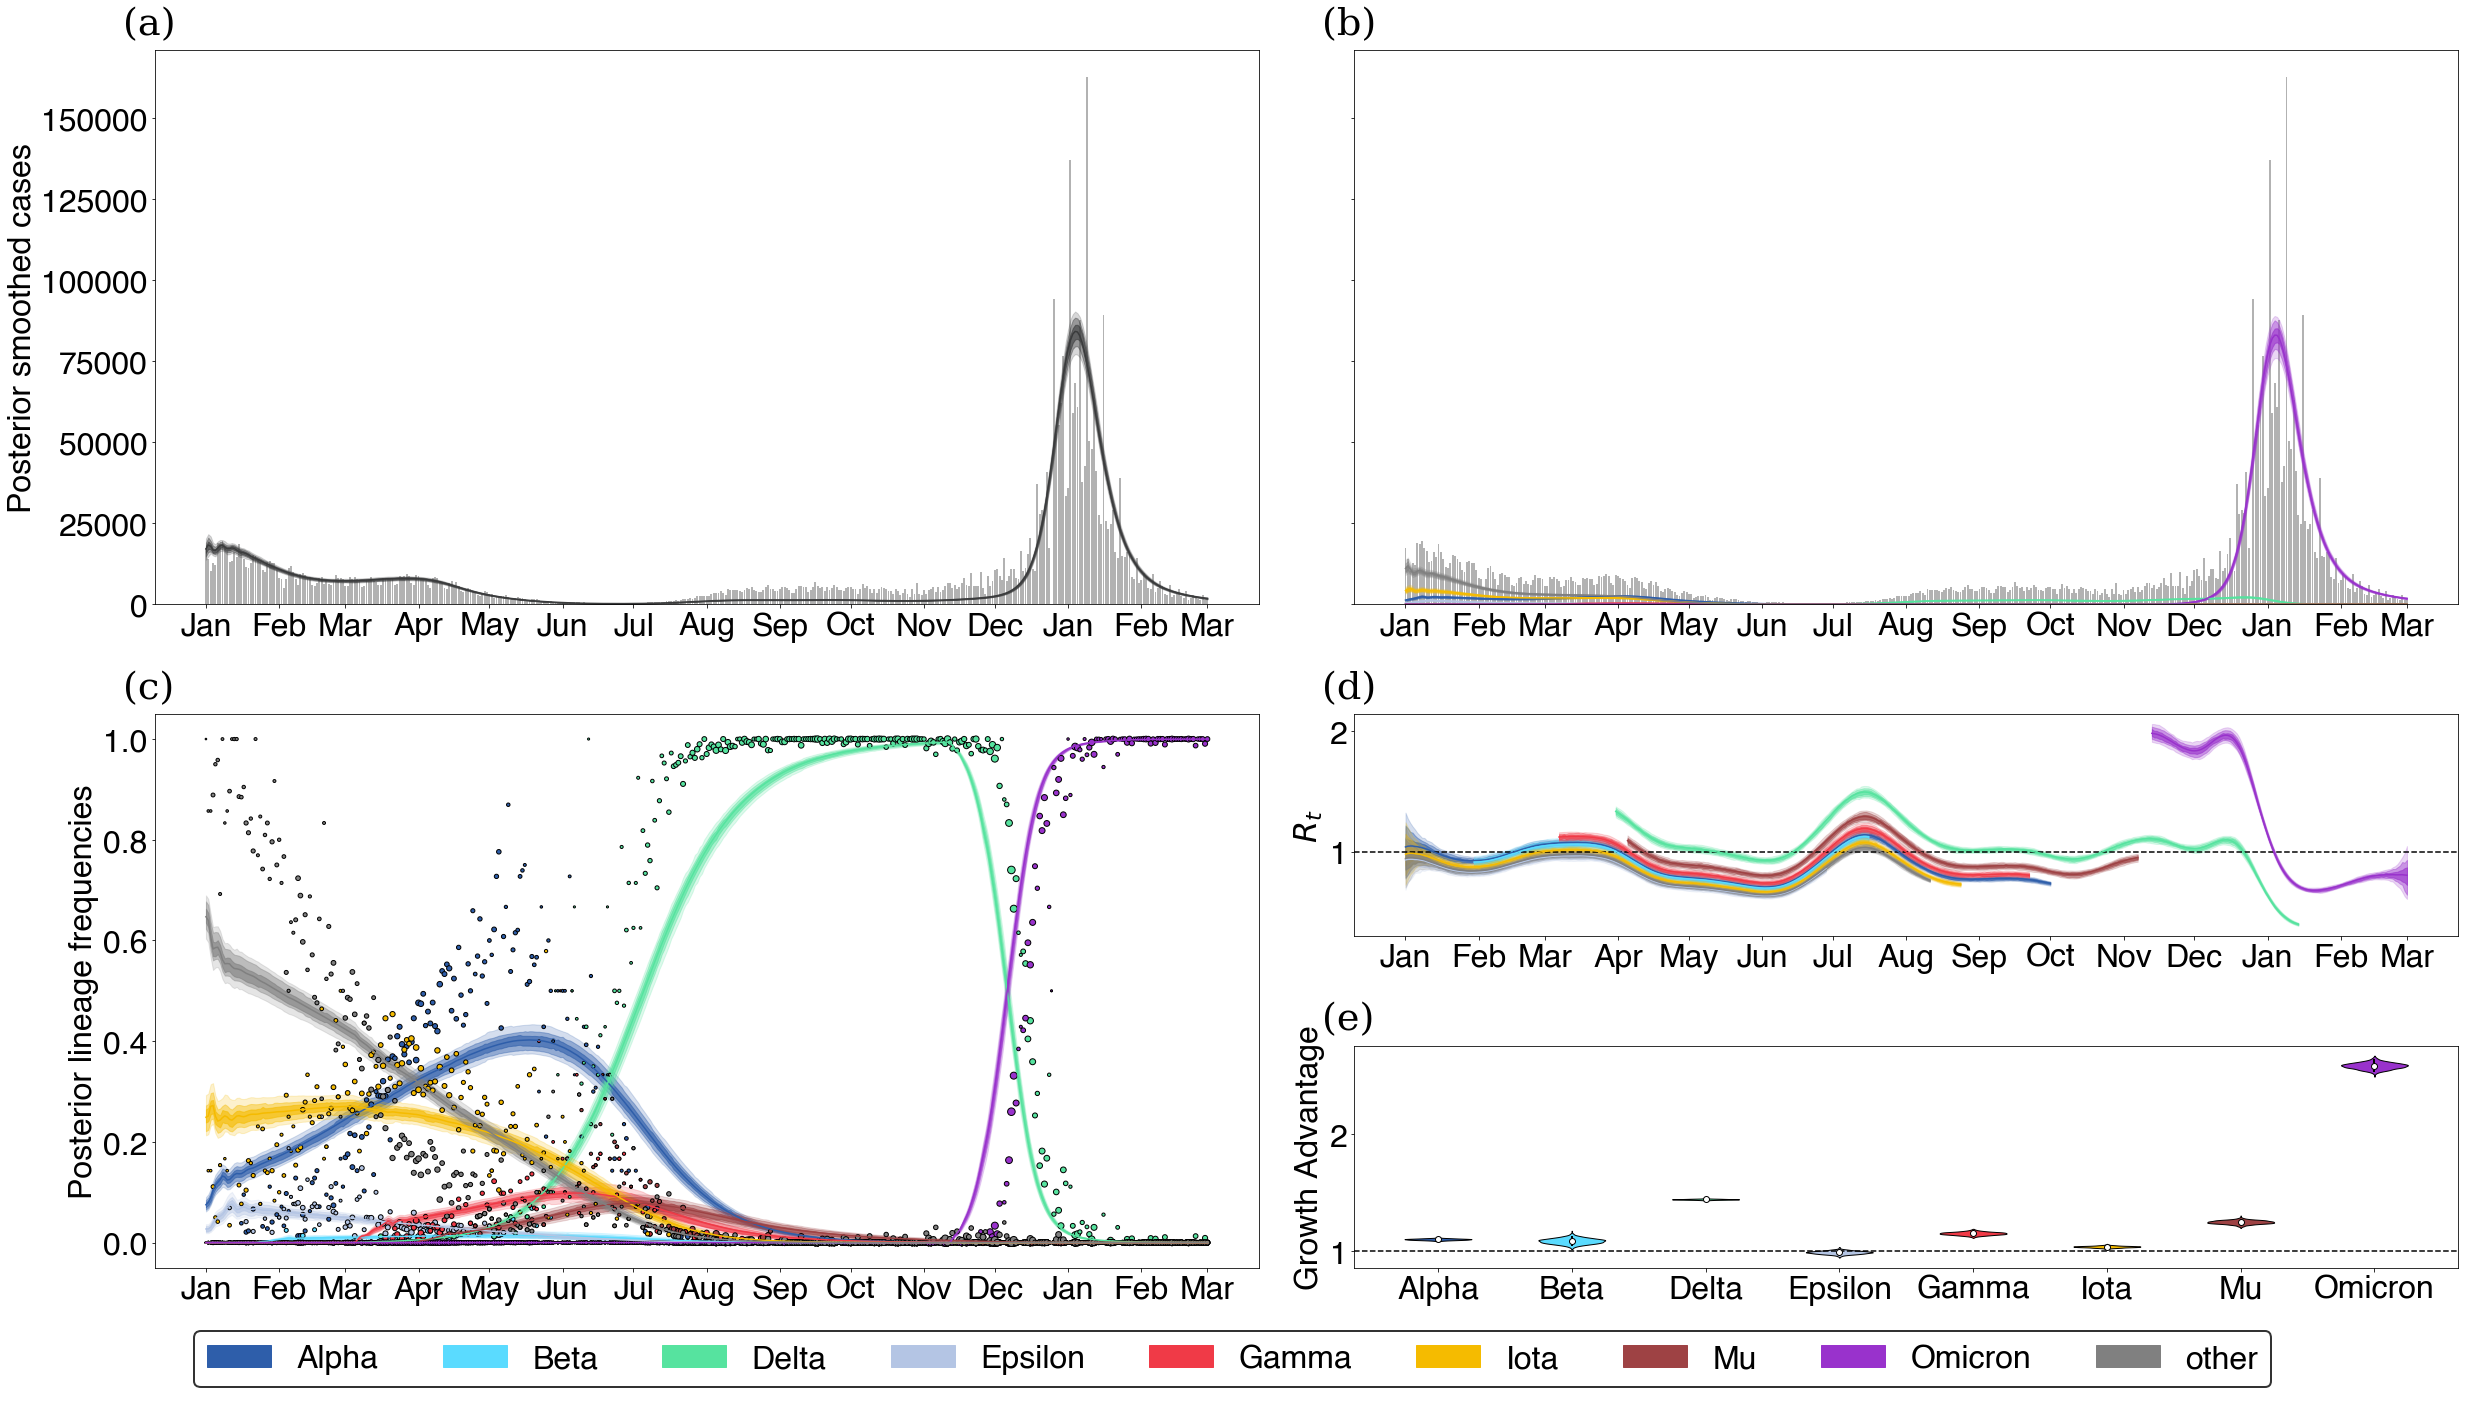
\includegraphics[width=\linewidth]{figs/fixed_growth_New-York.png}
  \caption{\textbf{Fitting the fixed growth advantage model to New York state data.}}%
  \label{fig:fixed_growth_New-York}
\end{figure}

\end{document}
